% \documentclass[a4]{scrartcl}

\documentclass[12pt,a4paper, usenames, dvipsnames]{scrartcl}
\usepackage{graphicx}
\usepackage{xcolor}


\usepackage[ngerman]{babel}
\usepackage[utf8]{inputenc}
\usepackage{mathtools}
\usepackage{amsmath}
\usepackage{amssymb}
\usepackage{geometry}
\usepackage{scrpage2}
\usepackage{tikz}
\usepackage{float}
\usepackage{verbatim}

\usepackage{subfigure}
\usepackage[center]{caption}


\pagestyle{plain}
% \clearscrheadfoot
\pagenumbering {arabic} 

\usepackage[backend=bibtex,style=numeric, citestyle = numeric]{biblatex}
\addbibresource{quellen.bib}

\usepackage[babel,german=guillemets]{csquotes}




\geometry{
  paper=a4paper, % Change to letterpaper for US letter
  top=1.5cm, % Top margin
  left=2cm, % Left margin
  right=3cm, % Right margin
  %showframe, % Uncomment to show how the type block is set on the page
}

\pagenumbering {arabic} 









\begin{document}



\begin{titlepage}
	\centering
	\vspace*{4cm}
	{\scshape\LARGE Technische Universität Dortmund \par}
	\vspace{1cm}
	{\scshape\Large Proposal \\
	(zur Bachelorarbeit) \par}
	\vspace{1.5cm}
	{\huge\bfseries  Gruppentheorie des 2x2x2 Zauberwürfels und dessen Lösungsalgorithmen \par}
	\vspace{2cm}
	{\Large\itshape Pina Kolling\par}
	\vfill
	betreut von\par
	Dr. Lukasz \textsc{Czajka}

	\vfill

% Bottom of the page
	{\large \today\par}
\end{titlepage}


\tableofcontents

\thispagestyle{empty} 



\newpage

\setcounter{page}{1} 

\section{Einleitung/Ausgangslage}

Meine Bachelorarbeit soll sich mit dem 2x2x2 Zauberwürfel und dessen Algorithmen zur Lösung befassen. Dabei handelt es sich um ein Drehpuzzle, das ein mathematisches Problem darstellt. \\ 
Im Folgenden werde ich die Terminologie und den Aufbau des Würfels erklären.\\
Terminologie:
\begin{figure}[h]
\centering
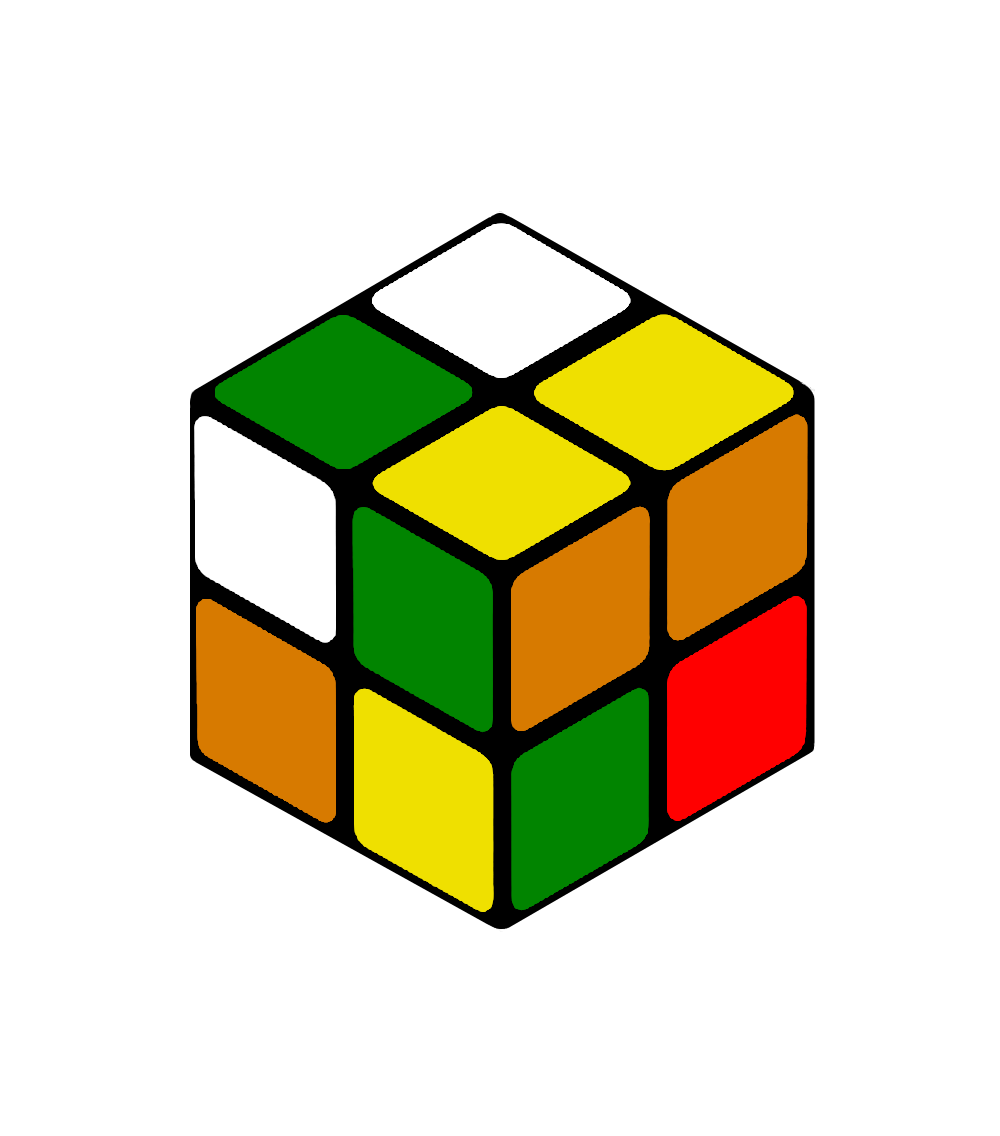
\includegraphics[scale=0.1]{2x2scrambled.png}
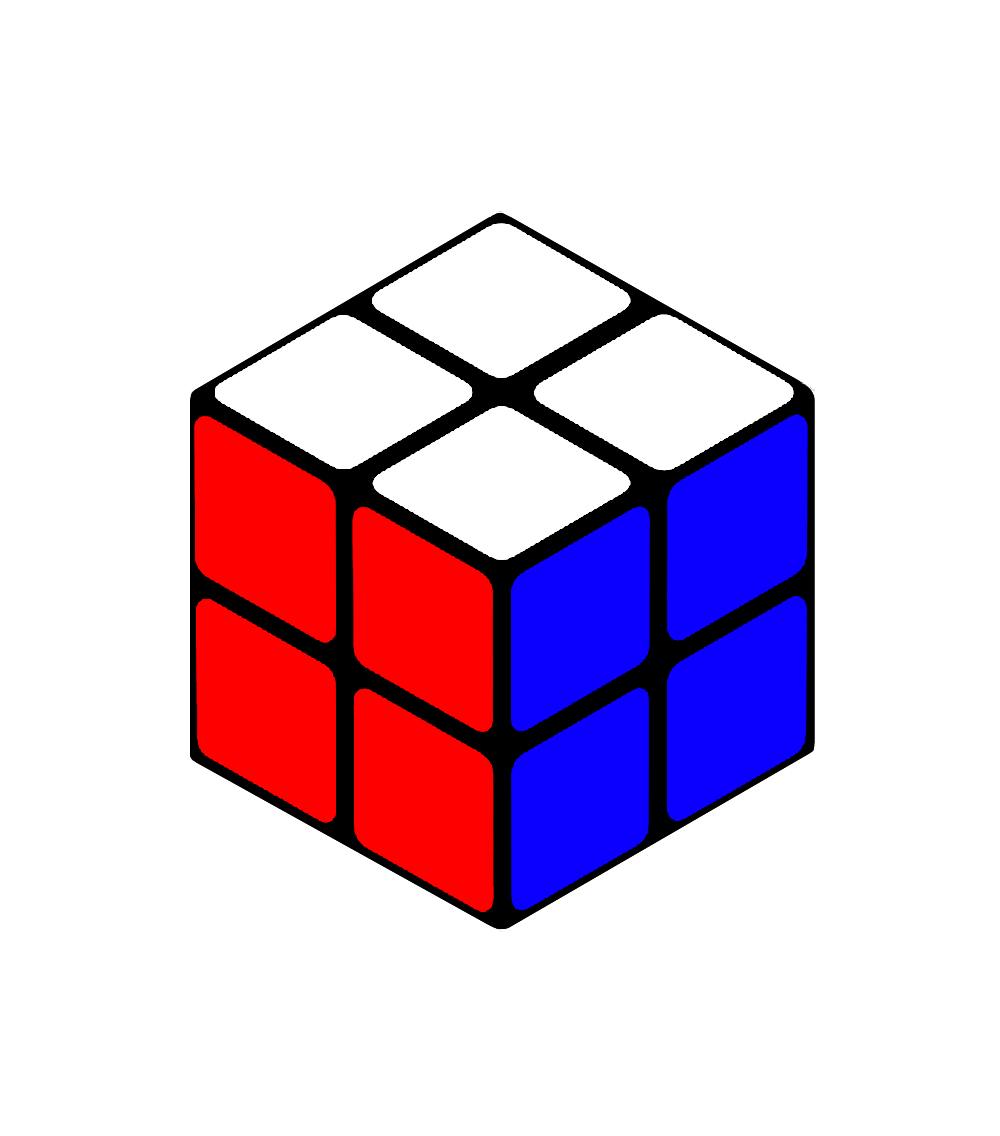
\includegraphics[scale=0.1]{2x2solved.png}
\caption{2x2x2 Zauberwürfel \\ (links in ungelöstem und rechts in gelöstem Zustand (Startkonfiguration)) \\
Der Zauberwürfel wird auch Würfel/Cube genannt.}
\end{figure}
\ \\
Bei der Startkonfiguration (auch Grundposition, Grundstellung) des 2x2x2 Würfels hat jede Seite 4 Farbflächen einer Farbe. Der Würfel ist dann gelöst. \\

\begin{figure}[h]
\centering
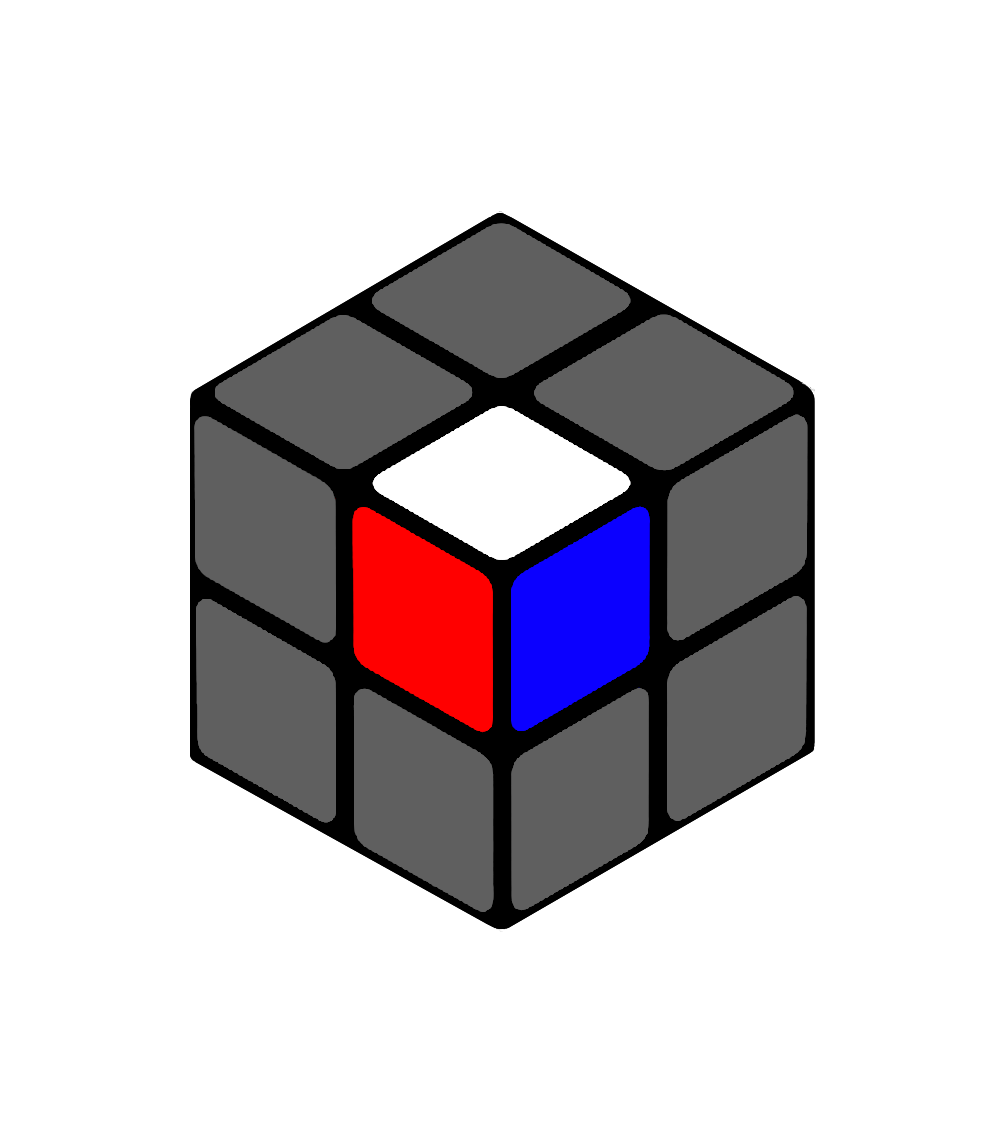
\includegraphics[scale=0.1]{2x2stein.png}
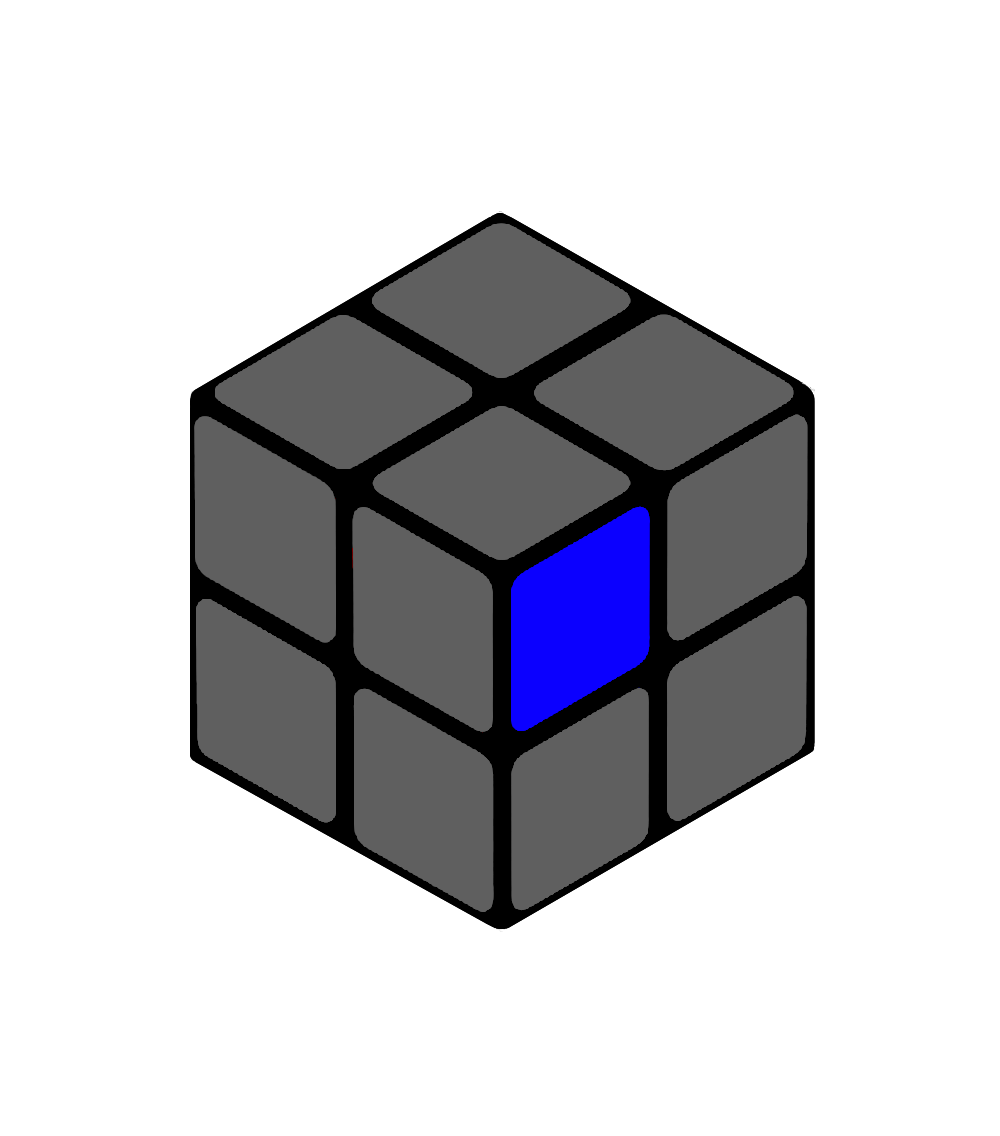
\includegraphics[scale=0.1]{2x2farbflaeche.png}
\caption{Ein 2x2x2 Würfel besteht aus acht (Eck-)Steinen (links), die jeweils drei Farbflächen (rechts) haben. Ein 2x2x2 Zauberwürfel hat also 24 Farbflächen.}
\end{figure} 
$\ $ \\
Die Ecksteine können sich in jeder Ecke befinden, also gibt es pro Eckstein 8 mögliche Positionen im Würfel. Da es 8 Ecksteine gibt, gibt es also $8! = 1 \cdot 2 \cdot 3 \cdot 4 \cdot 5 \cdot 6 \cdot 7 \cdot 8 = 40\, 320$ mögliche Positionen für die Ecksteine. \\
Außerdem können die Ecksteine gedreht sein, also verschiedene Farbflächen oben sein. Da die Steine aus 3 Farbflächen bestehen, können sie durch Rotationen theoretisch 3 verschiedene Ausrichtungen annehmen. Es gibt also $3^8$ Wege, wie die Ecksteine ausgerichtet sein können. \\
Somit ergibt es $3^8 \cdot 8!$ theoretisch mögliche Positionen für den Würfel. Das sind $264\, 539\, 520$ Positionen.\\
Es sind aber nicht alle dieser Positionen valide. Eine Position ist valide, wenn sie durch drehen der Seiten erreicht werden kann, ausgehend von der Startkonfiguration aus. \\

\begin{figure}[h]
\centering
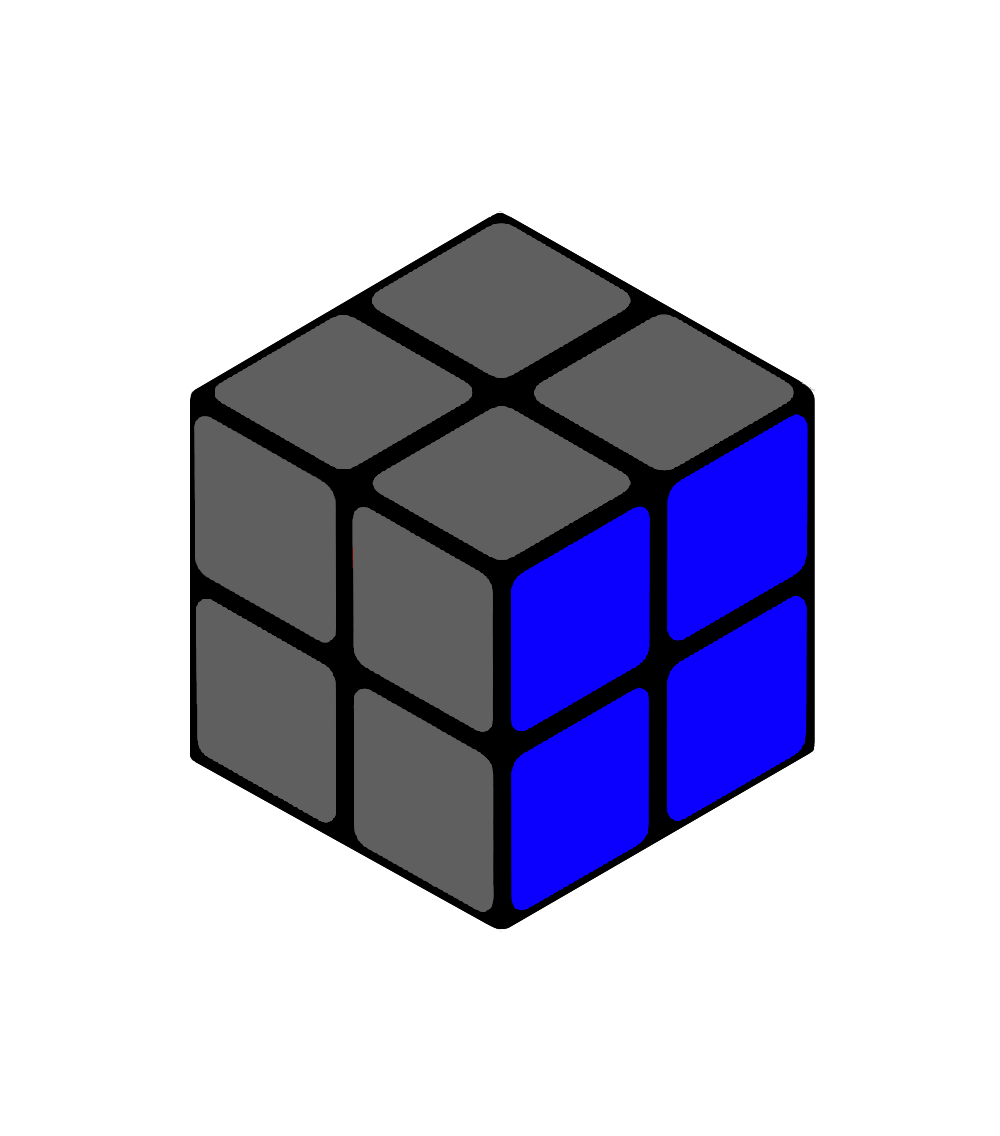
\includegraphics[scale=0.1]{2x2seite.png}
\caption{Der 2x2x2 und der 3x3x3 Zauberwürfel haben jeweils 6 Seiten.}
\end{figure}


\begin{figure}[h]
\centering
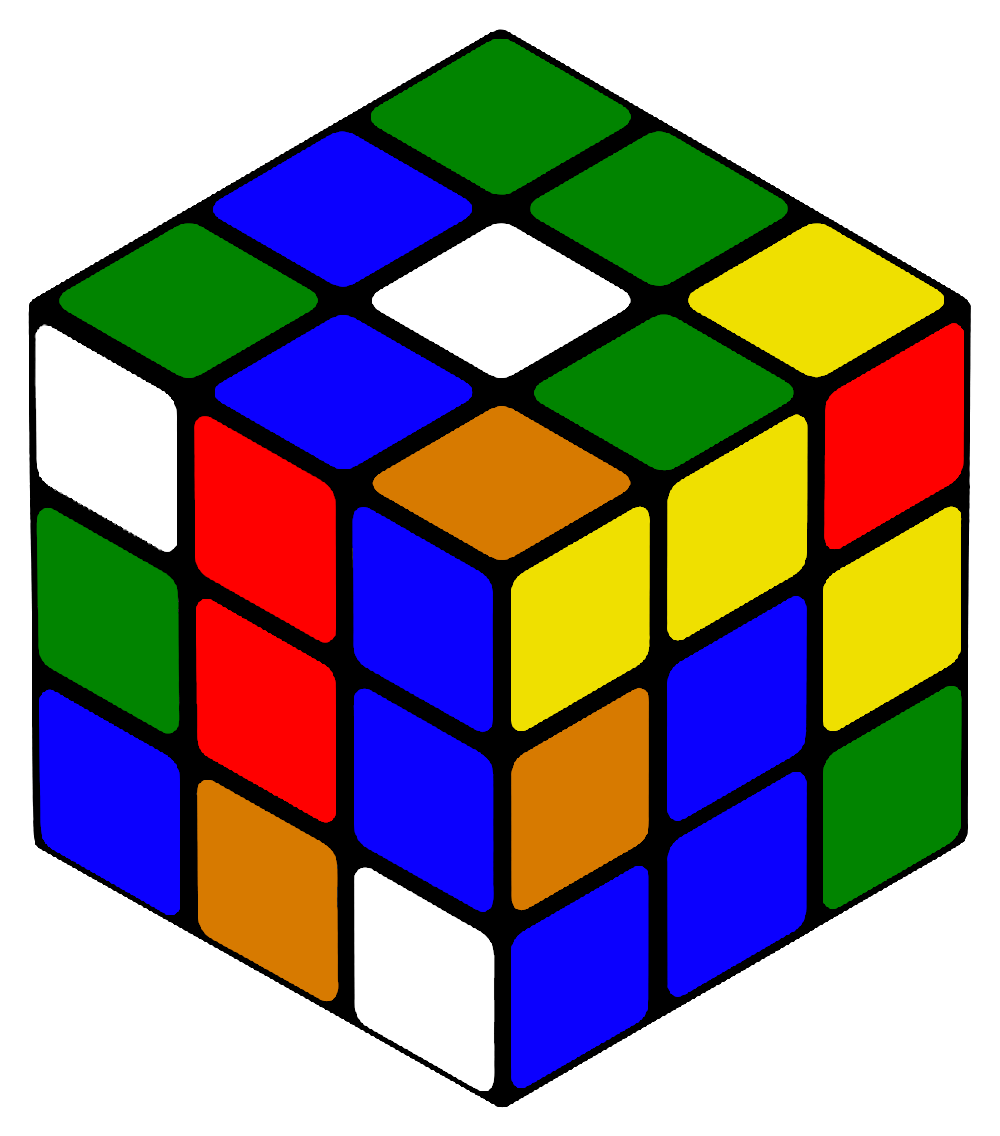
\includegraphics[scale=0.09]{3x3scrambled.png}
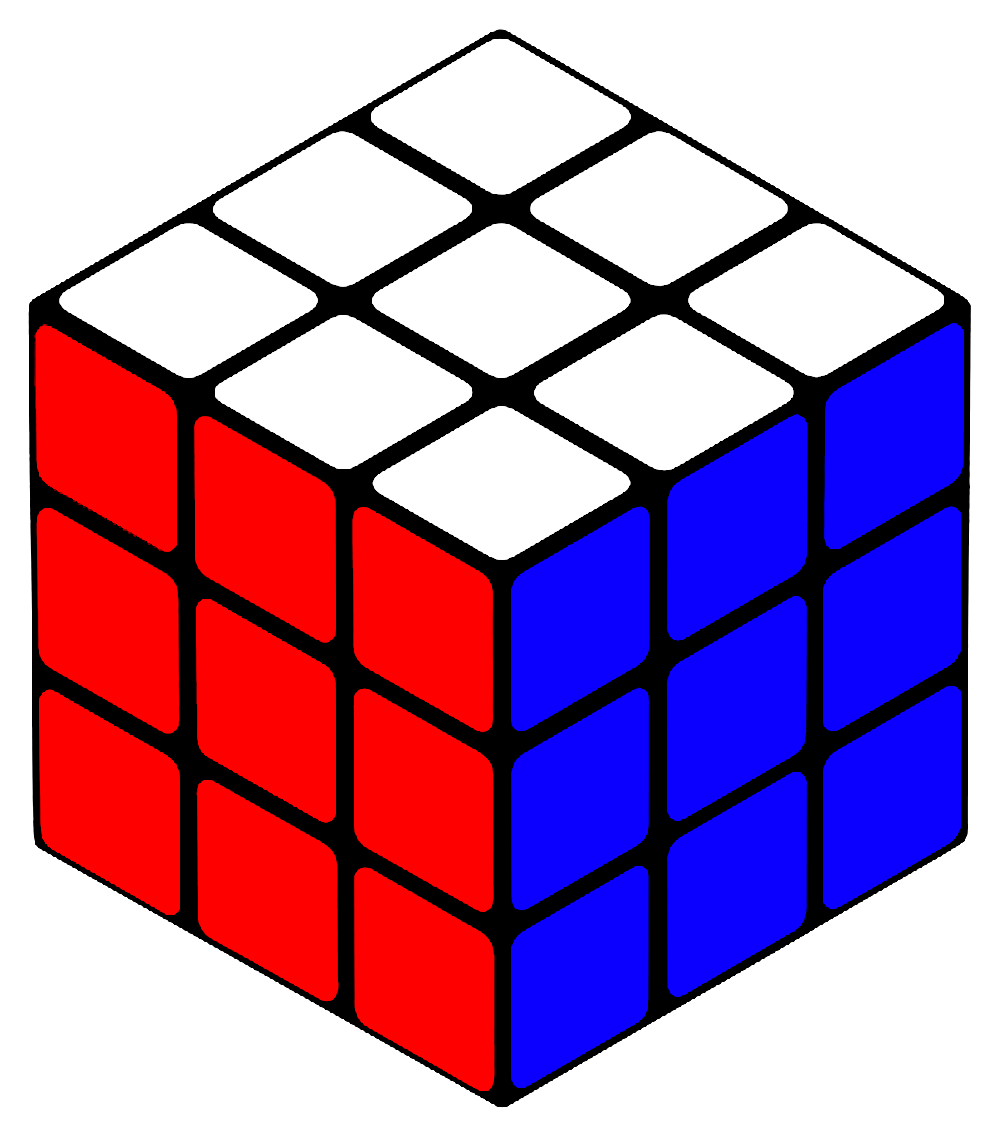
\includegraphics[scale=0.09]{3x3solved.png}
\caption{3x3x3 Zauberwürfel \\ (links in ungelöstem und rechts in gelöstem Zustand (auch Grundstellung))}
\end{figure}

\newpage
$\ $\\
Im Gegensatz zum 3x3x3 Würfel hat der 2x2x2 Würfel weder Mittelsteine, noch Kantsteine. \\
Das besondere an den Mittelsteinen des 3x3x3 Würfels ist, dass sie bei der Rotation der Seiten (also bei Zügen des Würfels) nicht verändert werden. Somit ist beim 3x3x3 Würfel die obere Seite immer fest zu stellen: Die obere Seite hat immer das weiße Mittelstück in der Mitte. \\
Beim 2x2x2 muss auch noch geprüft werden, ob die aktuelle Konfiguration nicht einer vermeintlich anderen Konfiguration entspricht, bei der nur eine andere Seite nach oben gehalten wird. \\
Die Rotation des gesamten Würfels ist bei dem 3x3x3 Würfel also eindeutig vorgegeben, während sie beim 2x2x2 Würfel gedreht werden kann. \\
\\

% Da der 2x2x2 Würfel keine Mittelsteine hat, so wie der 3x3x3, gibt es einige Positionen, die äquivalent zueinander sind (durch drehen des Würfels). \\
% Beispielsweise beschreibt \textit{ulf $\rightarrow$ dlf $\rightarrow$ dlb $\rightarrow$ ulb $\rightarrow$ ulf} ein Rotieren des kompletten Würfels nach vorne, wenn keine Züge gemacht werden. Dabei werden natürlich auch alle anderen Positionen mit rotiert. Der Stein \textit{urf} bewegt sich dabei beispielsweise auch mit: \textit{urf $\rightarrow$ drf $\rightarrow$ drb $\rightarrow$ urb $\rightarrow$ urb}. \\
% Im späteren Verlauf der Arbeit muss beachtet werden, dass dieser Würfel rotiert werden kann und es somit für die gleichen Steinpositionen verschiedene Optionen gibt, da der Würfel gedreht werden kann.

\newpage

\subsubsection*{Algorithmen}
Am 2x2x2 Zauberwürfel gibt es sechs verschiedene Drehseiten: oben, unten, links, rechts, vorne und hinten. Da der Würfel aber nur aus zwei Ebenen besteht, entspricht eine Drehung der oberen Ebene nach rechts, einer Drehung der unteren Ebene nach links. \\
Obwohl ich aber davon ausgehe, den kompletten Würfel beliebig zu rotieren, definiere ich die Drehungen der Ebenen für jede Ebene, damit die Algorithmen anschaulicher sind. Sonst entspräche ja eine Drehung der oberen Ebene im Uhrzeigersinn ($U$) einer dreifachen Drehung der unteren Ebene im Uhrziegersinn ($DDD$) mit anschließender Rotation des kompletten Würfels im Uhrzeigersinn. Es ist aber übersichtlicher, jede Ebenendrehung als einzelnen Zug dar zu stellen. \\
\\
\begin{tabular}{|c|l|}
\hline
Abkürzung & Beschreibung des Zugs \\
\hline
\hline
$U$ & Drehung der oberen Ebene im Uhrzeigersinn \\
\hline
$D$ & Drehung der unteren Ebene im Uhrzeigersinn \\
\hline
$R$ & Drehung der rechten Ebene im Uhrzeigersinn \\
\hline
$L$ & Drehung der linken Ebene im Uhrzeigersinn \\%
\hline
$F$ & Drehung der vorderen Ebene im Uhrzeigersinn \\
\hline
$B$ & Drehung der hinteren Ebene im Uhrzeigersinn \\
\hline
\end{tabular} \\
\\
Die Kürzel stehen für \textit{Up, Down, Right, Left, Front, Back}.  \\
\\
Die entsprechende Ebene wird im Uhrzeigersinn gedreht, wenn man auf diese Ebene schaut. Es wirkt also so, also würde man die untere Ebene gegen den Uhrzeigersinn drehen, wenn man von oben auf den Würfel schaut. 

\newpage

\section{Würfel als Gruppe}

\subsection*{Darstellung des 2x2x2 Zauberwüfels mit dem mathemtischen Konstrukt der Gruppe}

Die Definition einer Gruppe $(G, \circ)$ ist Grundlage für den folgenden Abschnitt:
\begin{itemize}
\item Abgeschlossenheit: $\forall a,b \in G.(a \circ b) \in G $
\item Assoziativität: $\forall a,b,c \in G.(a \circ b) \circ c = a \circ (b \circ c)$
\item Existenz eines neutralen Elements $n$: $\forall a \in G, \exists n \in G.n \circ a = a \circ n = a$ 
\item Existenz eines inversen Elements $a^{-1}$: $\forall a \in G, \exists a^{-1} \in G. a \circ a^{-1} = a^{-1} \circ a = n$ 
\end{itemize}
\ \\
Im folgenden setze ich die Definition der Gruppe des 3x3x3 Würfels aus dem Paper \glqq Group Theory and the Rubik's Cube\grqq \  von Janet Chen als Gruppe des 2x2x2 Würfels um. Die Gruppe von Janet Chen bezeichne ich als $(G_{3x3x3}, \circ)$, auch wenn Janet Chen sie als $(G, *)$ bezeichnet hat. Den Namen der Gruppe ändere ich aber, um klar zwischen dem 2x2x2 und dem 3x3x3 Würfel zu differenzieren. Das Symbol des Operators verändere ich, um Verwechslungen mit dem Multiplikationsoperator zu vermeiden. \\
\\ 
Die Gruppe des 2x2x2 Würfels nenne ich $(G_{2x2x2}, \circ)$. \\
\\
Die Menge $G_{2x2x2}$ besteht aus allen möglichen Zügen des Würfels. Beispielsweise die Drehung der oberen Ebene ist ein Zug. Ein Zug kann aber auch aus mehreren Drehungen bestehen, z.B. das Drehen der oberen Ebene, gefolgt von dem Drehen der rechten Ebene stellt ebenfalls einen Zug dar. \\
Wenn zwei Züge die gleiche Würfelposition hervorrufen, sind die beiden Züge "gleich". Beispielsweise eine Drehung um $180^{\circ}$ nach links oder nach rechts von einer Ebene führt zu dem gleihen Ergebnis und somit werden diese beiden Züge als gleich angesehen. \\
\\
Der Operator $\circ$ ist als Konkatenation zweier Züge definiert. Wenn $Z_1 \in G_{2x2x2}$ und $Z_2 \in G_{2x2x2}$ zwei Züge sind, dann bedeutet $Z_1 \circ Z_2$, dass zuerst $Z_1$ und dann $Z_2$ ausgeführt wird. (Außerdem gilt dann auch $Z_1 \circ Z_2 \in G_{2x2x2}$.) \\
Im folgenden werde ich begründen, wieso $(G_{2x2x2}, \circ)$ eine Gruppe ist, indem ich $(G_{2x2x2}, \circ)$ bezüglich der Gruppenkriterien untersuche: \\
\begin{itemize}
\item Abgeschlossenheit: \\ 
$\forall Z_1,Z_2 \in G_{2x2x2} .  (Z_1 \circ Z_2) \in G_{2x2x2} $ \\
\\
Die Gruppe $G_{2x2x2}$ ist abgeschlossen unter dem Operator $\circ$. Wenn $Z_1 $ und $Z_2$ Züge sind und somit Elemente von $G_{2x2x2}$, dann ist auch $Z_1 \circ Z_2$ ein Element der Gruppe, da alle Züge in $G_{2x2x2}$ enthalten sind. 

\item Assoziativität:\\ 
$\forall Z_1,Z_2,Z_3 \in G_{2x2x2}.(Z_1 \circ Z_2) \circ Z_3 = Z_1 \circ (Z_2 \circ Z_3)$ \\
\\
Die Züge $Z_i \in G_{2x2x2}$ können gruppiert werden und somit gilt die Assoziativität. \\
Um die Assoziativität zu zeigen, werde ich eine Schreibweise für das Ausführen der Züge einführen. Ich nenne einen bestimmten Stein im Würfel nun $s$. Beim Ausführen eines Zuges $Z$ schreibe ich nun $Z(s)$, um die neue Position des Steines zu erhalten. Die Positionen sind (wie oben beschrieben) 3-Buchstaben-Kürzel, bestehend aus $u, d, l, r, t, b$. \\
Wenn wir nun $Z_1 \circ Z_2 $ haben, wird zuerst $Z_1$ und dann $Z_2$ ausgeführt. $Z_1(s)$ bewegt den Stein s zu der Position $Z_1(s)$. Der Zug $Z_2$ bewegt den Stein dann zu der Position $Z_2(Z_1(s))$. Also gilt $Z_1 \circ Z_2 = Z_2(Z_1(s))$. \\
\\
Nun muss noch $(Z_1 \circ Z_2) \circ Z_3 = Z_1 \circ (Z_2 \circ Z_3)$ gezeigt werden. Ich zeige also, dass sich $(Z_1 \circ Z_2) \circ Z_3$ und $Z_1 \circ (Z_2 \circ Z_3)$ beide zu $Z_3(Z_2(Z_1(s))$ umformen lassen: \\
\begin{align*}
& (Z_1 \circ Z_2) \circ Z_3  \\
\Rightarrow (&(Z_1 \circ Z_2) \circ Z_3)(s) \\
= & Z_3(Z_1 \circ Z_2)(s)) \\
= & Z_3(Z_2(Z_1(s)))  
\end{align*}
\begin{align*}
&Z_1 \circ (Z_2 \circ Z_3) \\
\Rightarrow (&Z_1 \circ (Z_2 \circ Z_3))(s) \\
= (&Z_2 \circ Z_3)(Z_1(s)) \\
= \ \ & Z_3(Z_2(Z_1(s)))  
\end{align*}
Somit ist $(G_{2x2x2}, \circ)$ assoziativ.

\item Existenz eines neutralen Elements $N$:  \\
$\forall Z_1 \in G_{2x2x2}, \exists N \in G_{2x2x2}.N \circ Z_1 = Z_1 \circ N = Z_1$ \\
\\
Das neutrale Element $N$ muss aus der Menge $G_{2x2x2}$ der Züge sein und es muss gelten: $N \circ Z_1 = Z_1 \circ N = Z_1$. Somit ist das neutrale Element der Gruppe $(G_{2x2x2}, \circ)$ der \glqq leere \grqq \ Zug. Es werden also keine der Ebenen des Würfels gedreht. Wenn man also einen Zug $Z$ ausführt und dann den Zug $N$, bedeutet das so viel wie \glqq erst $Z$ ausführen und dann nichts \grqq , was das gleiche ist wie $Z$ auszuführen.


\item Existenz eines inversen Elements $Z_1^\prime$: \\ 
$\forall \  Z_1 \in G_{2x2x2},\ \exists \  Z_1^\prime \in G_{2x2x2}.  \ \ Z_1 \circ Z_1^\prime = Z_1^\prime \circ Z_1 = N$  \\
\\
Da $Z$ ein Zug ist, kann man diesen auch rückgängig machen. Man muss die einzelnen Ebenenrotationen nur rückwärts und von hinten durchführen, um den Zug zu invertieren. Dann gilt $Z_1 \circ Z_1^\prime = Z_1^\prime \circ Z_1 = N$.
\end{itemize}
Somit ist $(G_{2x2x2}, \circ)$ eine Gruppe. \\
Damit $(G_{2x2x2}, \circ)$ eine kommutaive Gruppe (oder Abelsche Gruppe) ist, muss zusätzlich noch die Kommutativität gelten. \\
Dies ist nicht der Fall, da beispielsweise eine Rotation der oberen Ebene nach rechts und eine Rotation der rechten Ebene nach unten in umgekehrter Reihenfolge ein anderes Ergebnis haben. Es gilt also nicht $\forall \  Z_1, Z_2 \in G_{2x2x2}. Z_1 \circ Z_2 = Z_2 \circ Z_1$. Der $\circ$-Operator der Gruppe ist also nicht kommutativ. \\
\\

\section{Konfiguration des Würfels}
Die Konfiguration des Würfels, also die Position/Verdrehung des Würfels setzt sich aus zwei Parametern zusammen: \\
\begin{itemize}
\item Position der Ecksteine (angegeben als $\sigma$)
\item Ausrichtung der Ecksteine (angegeben als $x_i$)
\end{itemize}
Also kann die Konfiguration des Würfels als ein 2-Tupel geschrieben werden: $(\sigma, x)$. \\
\\
Der Würfel kann aber auch komplett gedreht werden, ohne Züge auszuführen.

\subsection*{Positionen im Würfel und Zykel}

Um die Übergänge der Würfelsteine als Funktion darzustellen, definiere ich eine bijektive Funktion $\sigma$ für jede Rotation. $\sigma$ bildet jede der Würfelpositionen auf die neue Position ab. \\
\\
Die Würfelpositionen habe ich wie folgt eingeteilt: \\
\begin{figure}[H]
\centering
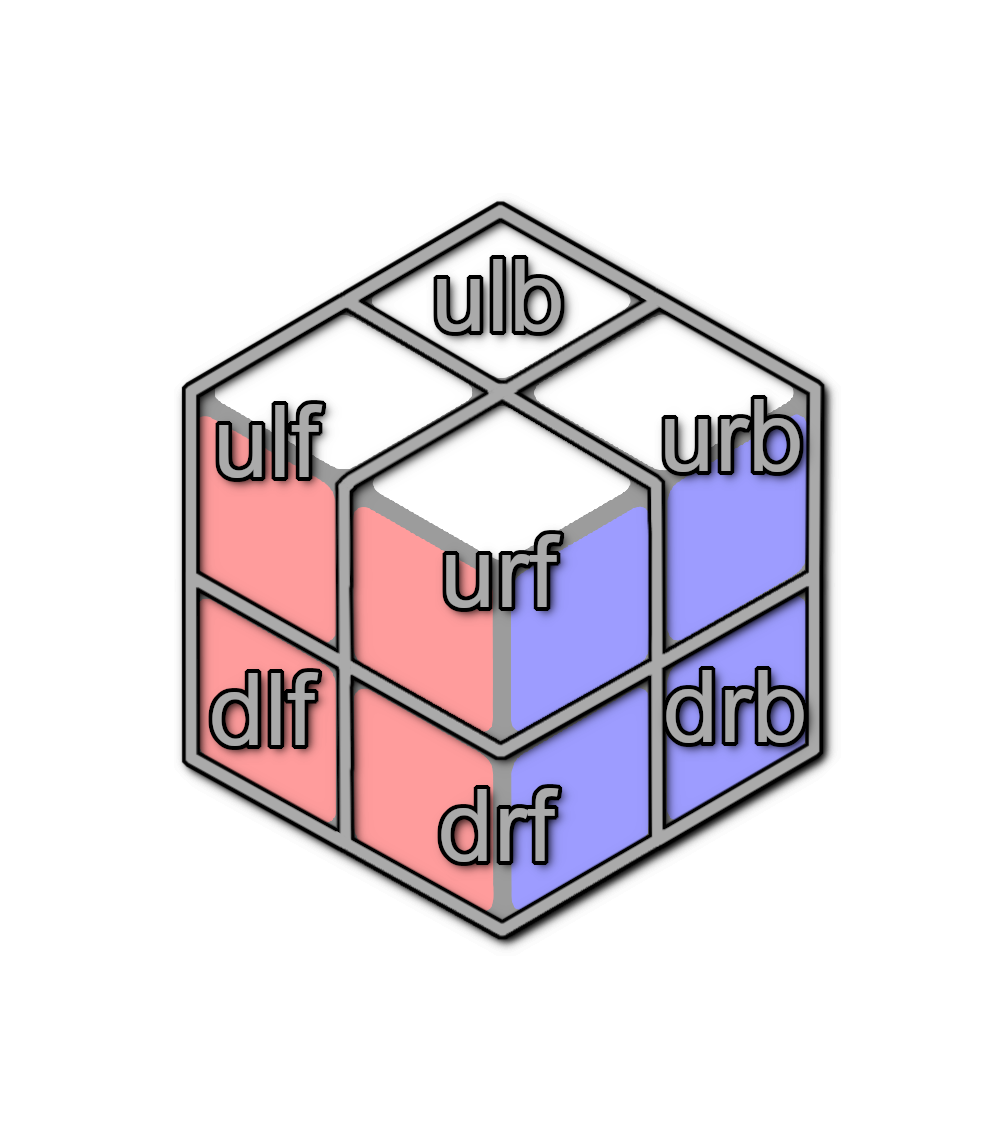
\includegraphics[scale=0.15]{caged_positions.png} \\
\caption{Die einzelnen Steinpositionen werden mit den Kürzeln benannt, die \textit{up, down, left, right, front und back} beschreiben.}
\end{figure}

\begin{figure}[H]
\centering
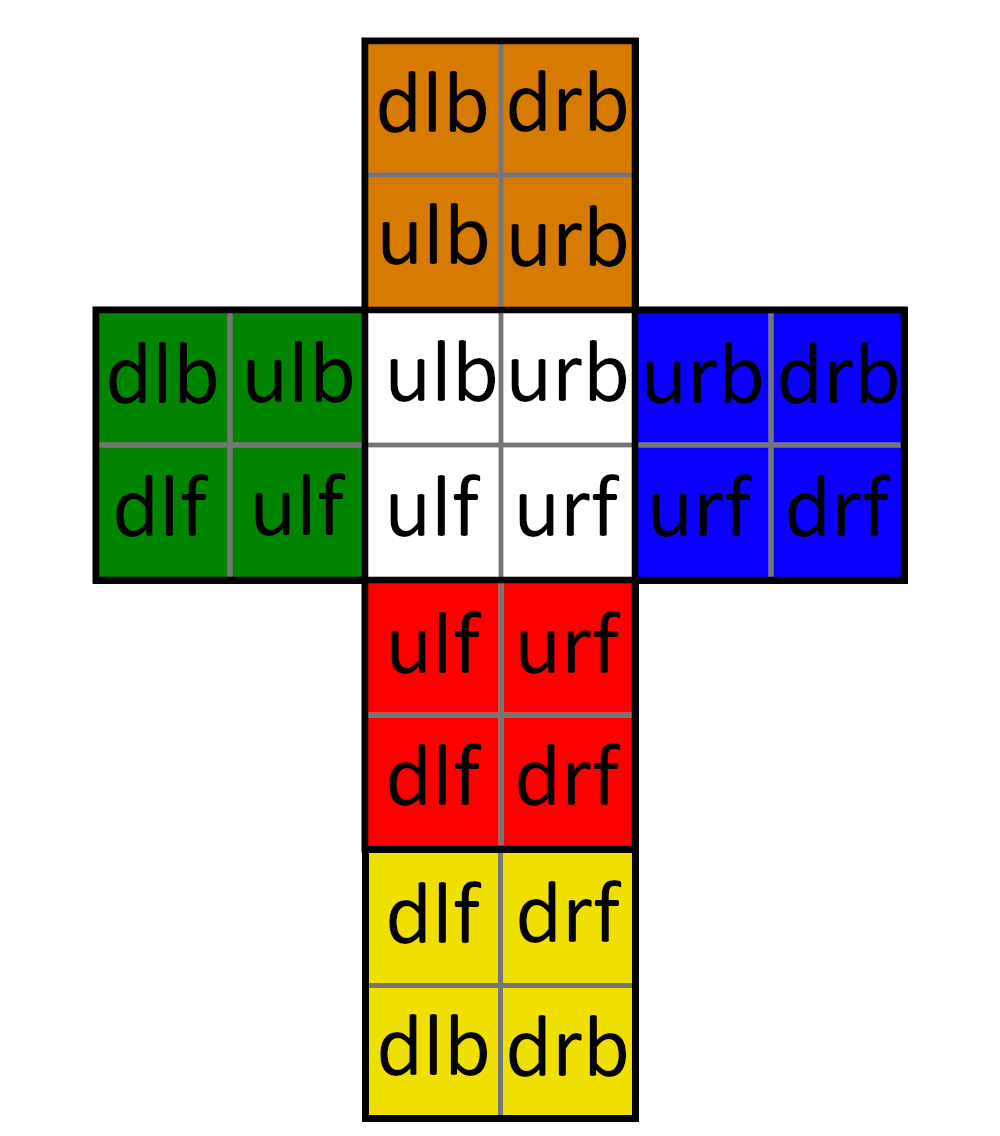
\includegraphics[scale=0.15]{foldedout_cage.png}
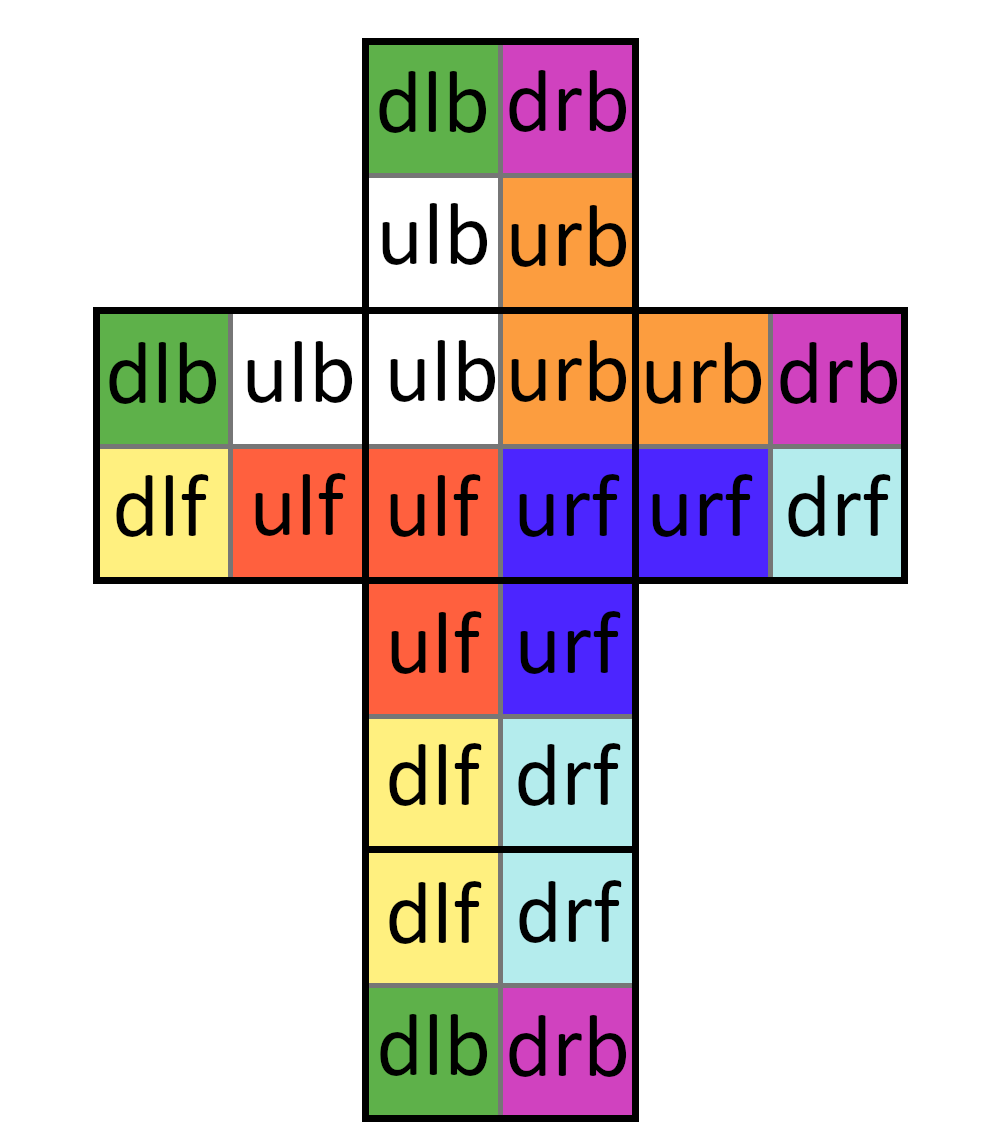
\includegraphics[scale=0.15]{foldedout_cage_color.png}
\end{figure}
\ \\
\\
Ich ordne jeder Steinposition einen einzigartigen Namen zu, um mich darauf zu beziehen. Dabei gehe ich davon aus, dass die weiße Seite in der Startkonfiguration oben ist. Die Steinposition beschreibe ich mich 3 Buchstaben, die aus den Kürzeln \textit{u, d, l, r, f, b} bestehen. Diese Kürzel stehen für \textit{up, down, left, right, front, back}. \\
Somit heißt die Steinposition oben links also \textit{ulf} (für up, left und front). 
\\
\\
Nun definiere ich $\sigma_U$ für eine Drehung der oberen Ebene um 90$^\circ$ im Uhrzeigersinn: \\
Ich beschreibe $\sigma_U$ ausführlich und gebe verschiedene Schreibweisen an. Die weiteren Drehungen funktionieren dann analog. \\
\\
Die Drehung der oberen Ebene sieht grafisch dargestellt so aus: \\
\begin{figure}[H]
\centering
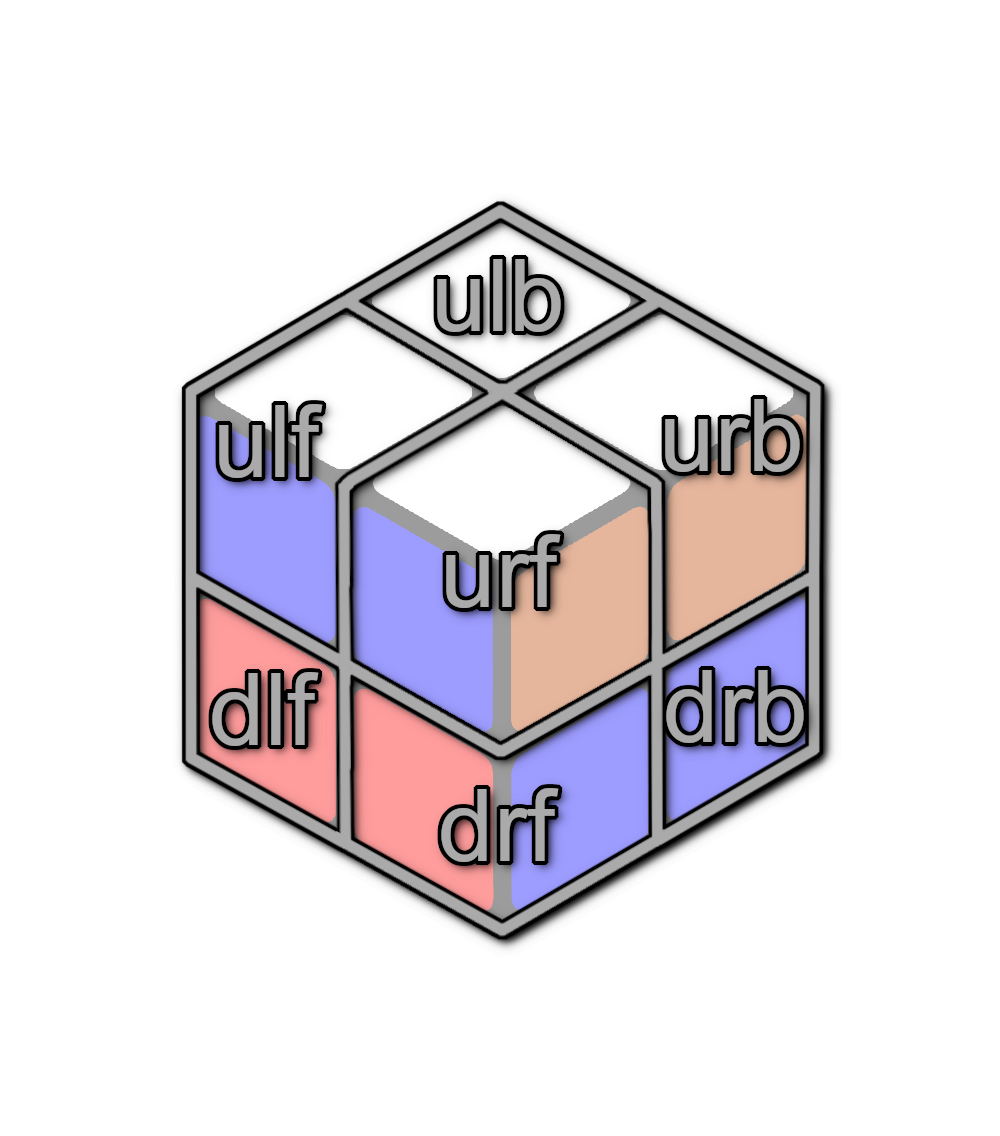
\includegraphics[scale=0.13]{caged_spin.png}
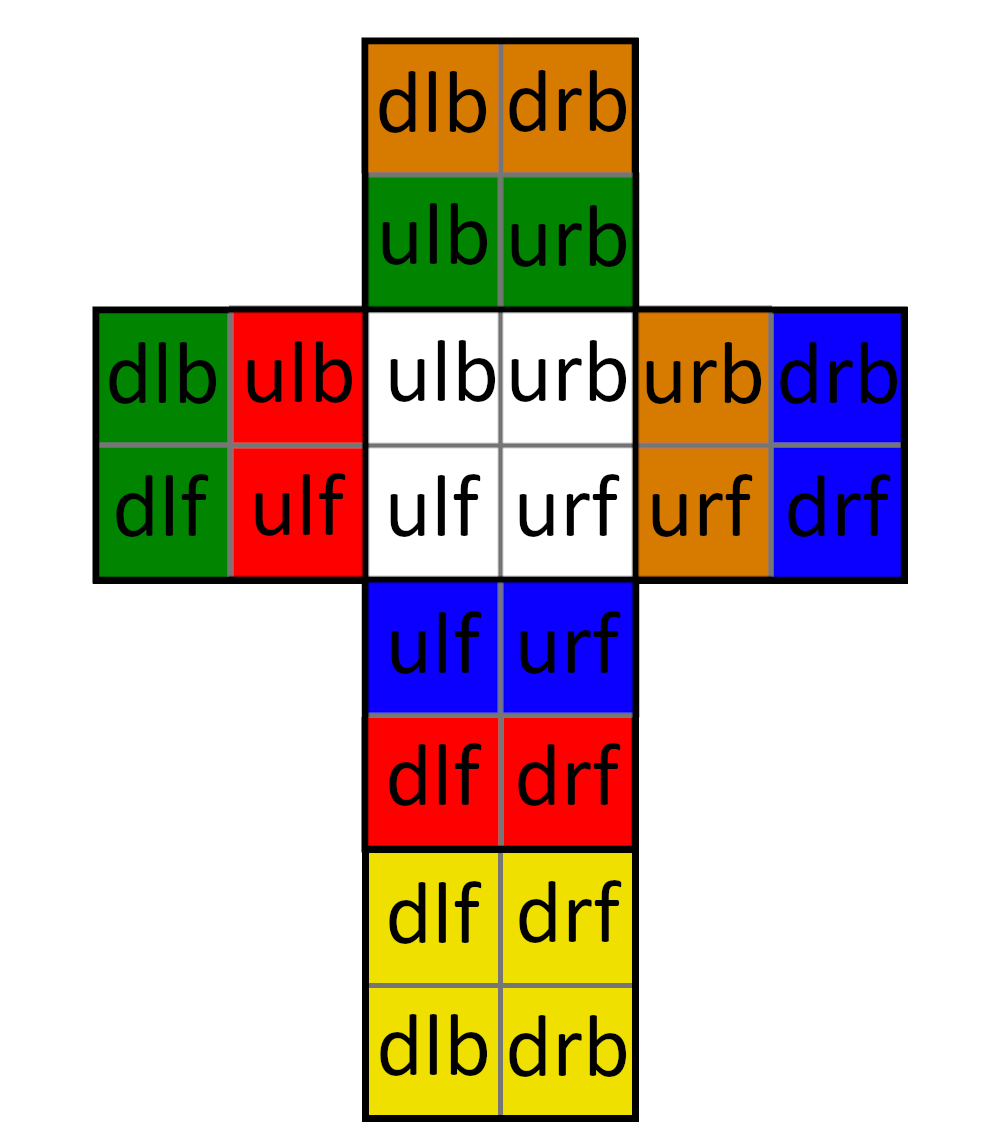
\includegraphics[scale=0.13]{foldedout_spin.png}
\end{figure}
\ \\
$\sigma_U(ulf)=ulb$ \ \ \ \ \ \ \ \ $\sigma_U(ulb)=urb$ \ \ \ \ \ \ \ \ $\sigma_U(urb)=urf$ \ \ \ \ \ \ \ \ $\sigma_U(urf)=ulf$ \\
$\sigma_U(dlf)=dlf$ \ \ \ \ \ \ \ \ $\sigma_U(dlb)=dlb$ \ \ \ \ \ \ \ \ \ $\sigma_U(drb)=drb$ \ \ \ \ \ \ \ \ $\sigma_U(drf)=drf$ \\
\\
Das kann man auch in der Form $i \mapsto j$ schreiben: \\
\\
$ulf \mapsto ulb$ \ \ \ \ \ \ \ \ $ulb \mapsto urb$ \ \ \ \ \ \ \ \ $urb \mapsto urf$ \ \ \ \ \ \ \ \ $urf \mapsto ulf$ \\
$dlf \mapsto dlf$ \ \ \ \ \ \ \ \ $dlb \mapsto dlb$ \ \ \ \ \ \ \ \ \ $drb \mapsto drb$ \ \ \ \ \ \ \ \ $drf \mapsto drf$ \\
\\
Daraus entstehen folgende Zykel: $\sigma_U = \ (ulf \ ulb \ urb \ urf)\ (dlf)\ (dlb)\ (drb)\ (drf)$ \\ \\
Die Zykel mit nur einem Element müssen nicht aufgeschrieben werden. Dann ergibt sich $\sigma_U = \ (ulf \ ulb \ urb \ urf)$, was den Zykel beschreibt, in dem die Steine rotiert werden, wenn die obere Ebene gedreht wird. \\
\\
Die Drehungen der anderen Ebenen können durch folgende Zykel beschrieben werden: \\
\begin{align*}
\sigma_U & =\ (ulf \ ulb \ urb \ urf) \\
\sigma_D & =\ (dlf \ drf \ drb \ dlb) \\
\sigma_F & =\ (ulf \ urf \ drf \ dlf) \\
\sigma_B & =\ (ulb \ dlb \ drb \ urb) \\
\sigma_L & =\ (ulb \ ulf \ dlf \ dlb) \\
\sigma_R & =\ (urb \ drb \ drf \ urf) \\
\end{align*}
Die Identitätspermutation schreibe ich als $\sigma = 1$.


\subsection*{Ausrichtung der Steine}
Der 2x2x2-Würfel besteht aus 8 Ecksteinen, die jeweils 3 Farbflächen haben. Somit hat jeder Stein 3 mögliche Ausrichtungen. \\
Um die Ausrichtung der Steine zu erkennen, bekommen Würfelpositionen an einer Farbfläche einer Nummer zugeordnet. Dafür habe ich die weißen und die gelben Seiten markiert und nummeriert. Auf diese Nummern beziehe ich mich als $x_i \in \lbrace 1, 2, 3, 4, 5, 6, 7, 8 \rbrace$ mit $x_1$ als Position 1, $x_2$ als Position 2, usw.
\begin{figure}[H]
\centering
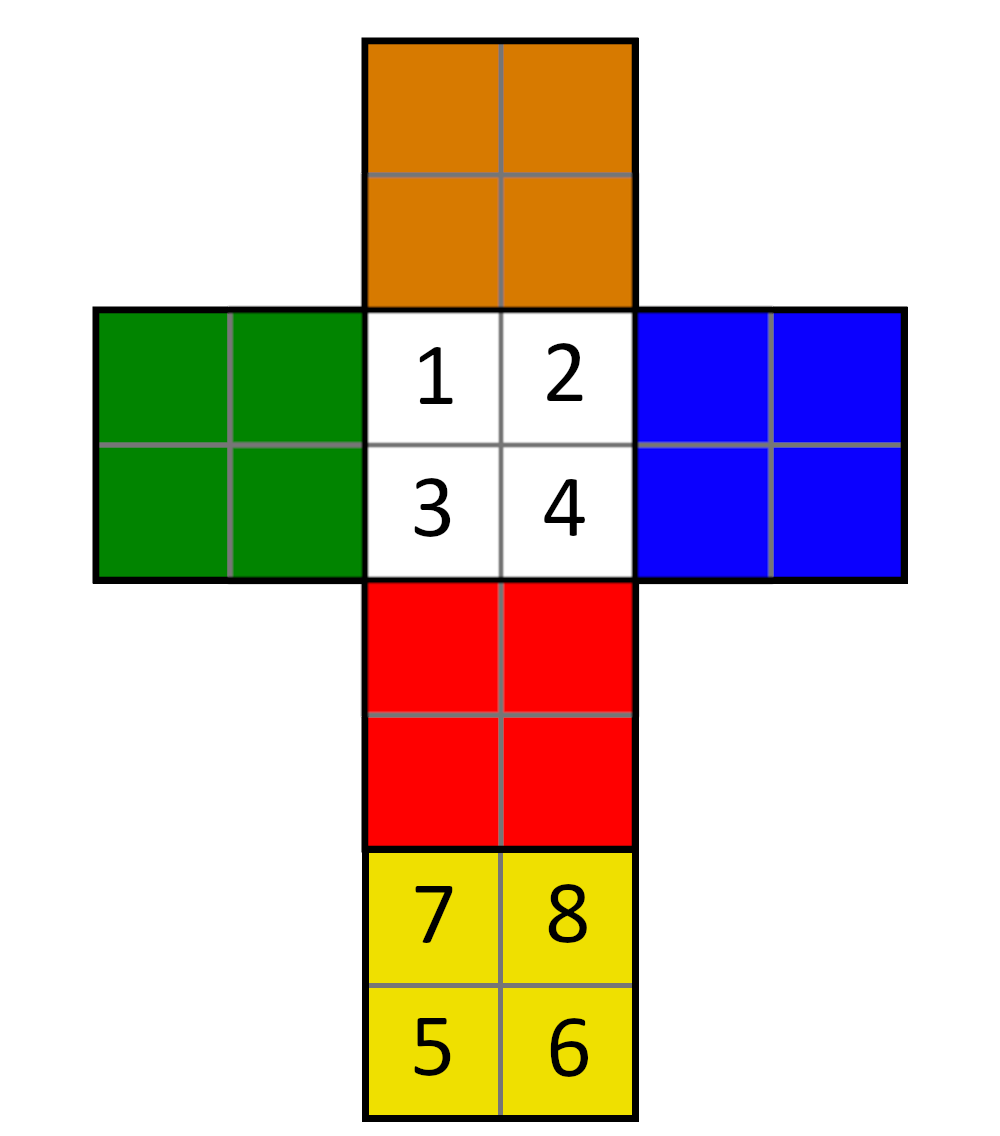
\includegraphics[scale=0.1]{foldedout_numbers.png}
\end{figure}
\ \\
Außerdem bekommt jeder Stein an jeder Farbfläche eine Zahlenzuordnung. Da jeder Stein 3 Ausrichtungen haben kann, nummeriere ich mit 0, 1 und 2. Ich beginne mit der weißen/gelben Fläche bei 0 und zähle dann im Uhrzeigersinn die Flächen. \\
\begin{figure}[H]
\centering
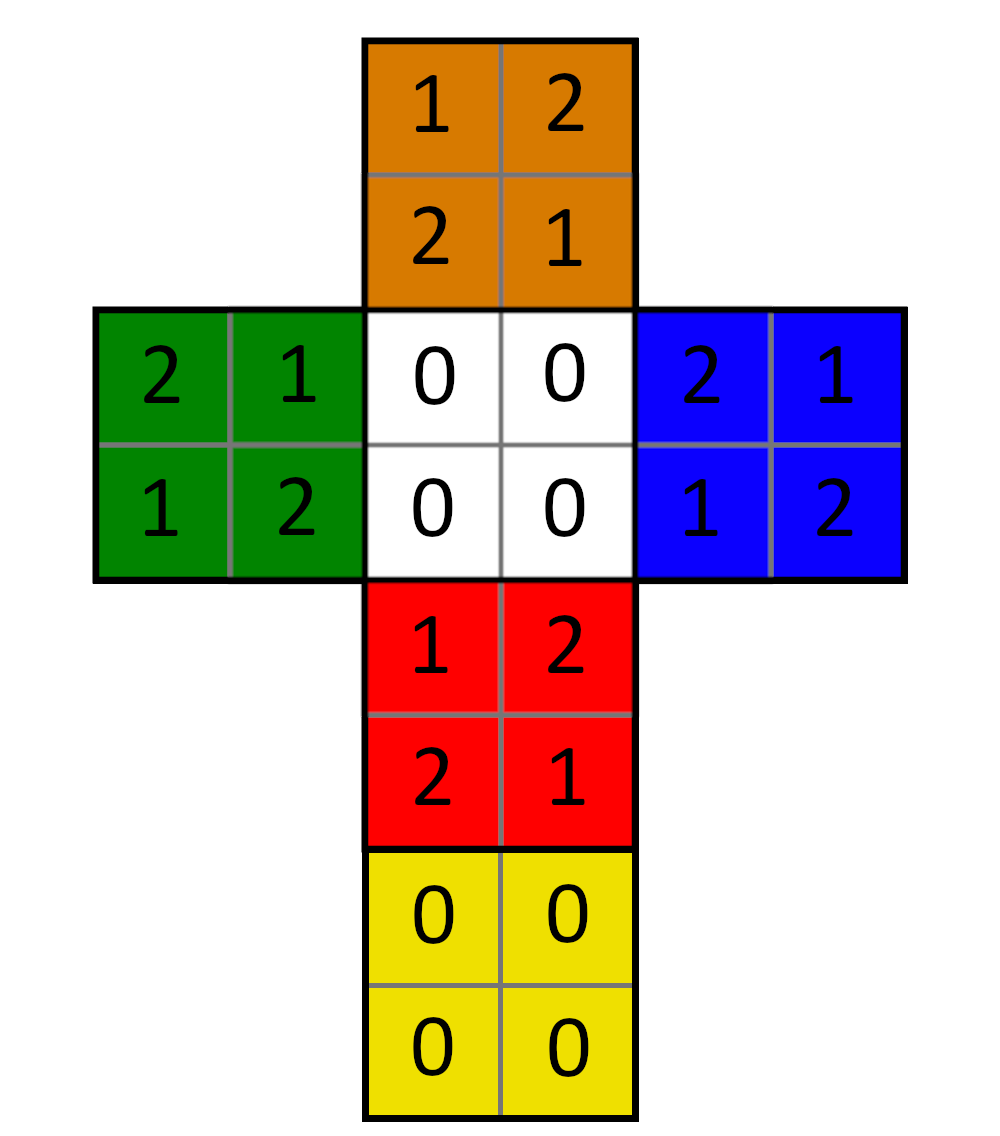
\includegraphics[scale=0.1]{foldedout_012.png}
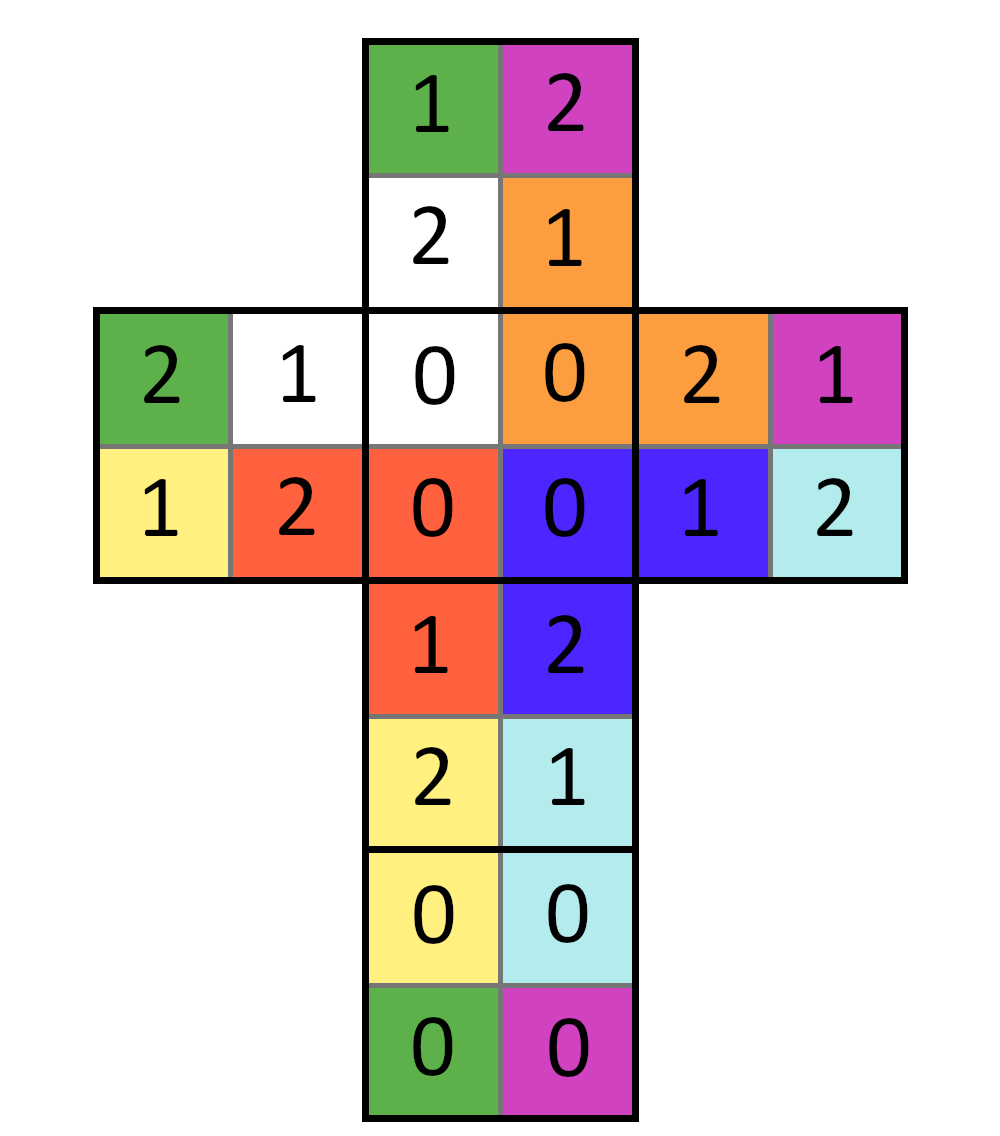
\includegraphics[scale=0.1]{foldedout_c_012.png}
\end{figure}
\ \\
In der Startkonfiguration sind alle $x_i = 0$, also $x=(0, 0, 0, 0, 0, 0, 0, 0)$. Das schreibe ich kurz als $x=0$.\\
\ \\
Nun stelle ich dar, wie sich die Nummerierung der Farbflächen verändert, wenn der Zug $R$ ausgeführt wird. $R$ ist eine Rotation der rechten Ebene um 90$^\circ$ im Uhrzeigersinn. \\
Die Nummerierungen der Position ($x$) bleiben an der gleichen Position, die Nummerierungen ($0, 1, 2$) der Farbflächen ändern sich mit Rotation der Ebene und ermöglichen so eine Zuordnung der Ausrichtung der Ecksteine. \\
Die linke Seite der Würfels wird dabei nicht beeinträchtig, also sind die Flächen an den Positionen $x_1, x_3, x_5, x_7$ alle 0. \\
Die anderen Positionen haben nun aber andere Farbflächen: \\
$x_2 = 2$ \ \ \ \ $x_4 = 1$ \ \ \ \ $x_6 = 1$ \ \ \ \ $x_8 = 2$  \\
Also $x = (0, 2, 0, 1, 0, 1, 0, 2)$ nach dem Zug $R$. \\
\begin{figure}[H]
\centering
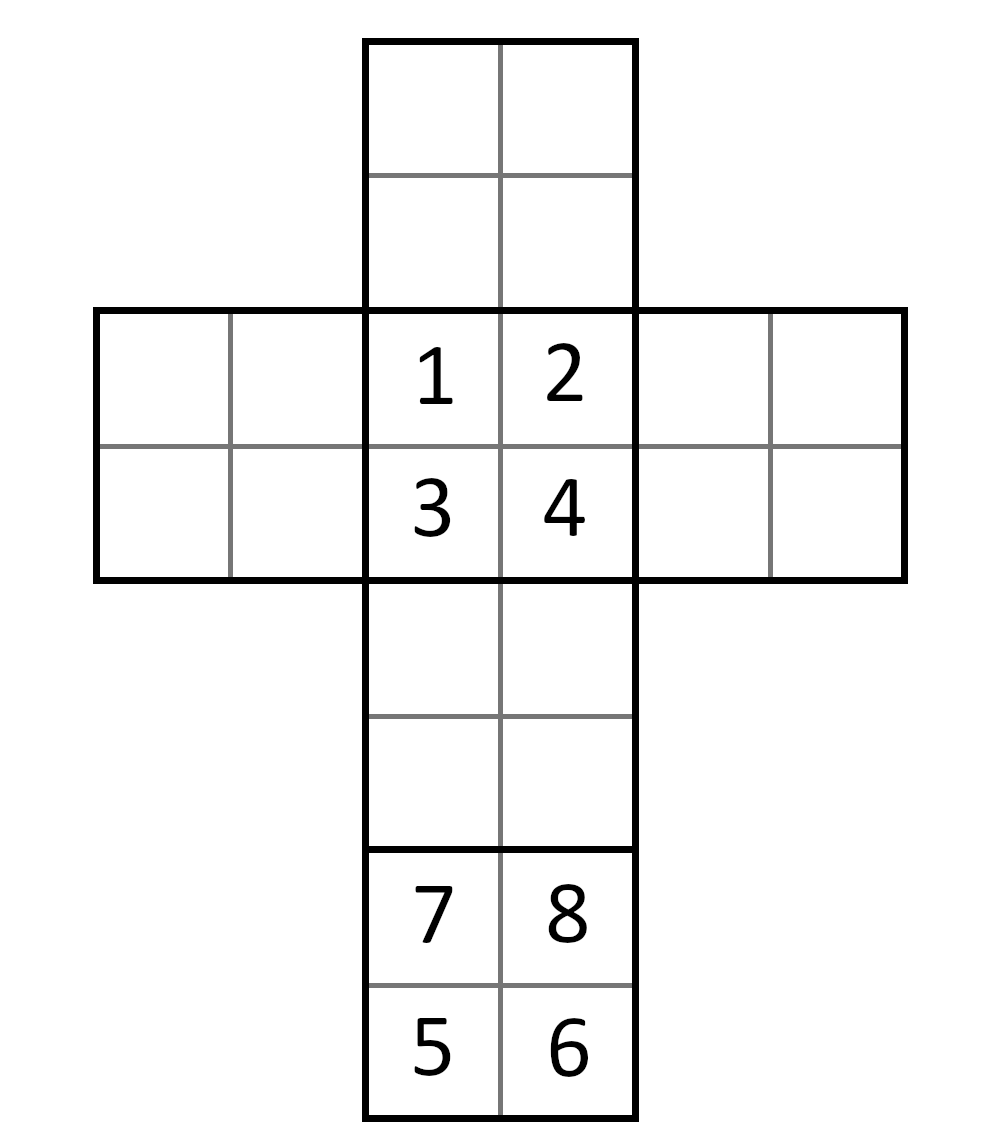
\includegraphics[scale=0.1]{foldedout_012_white.png}
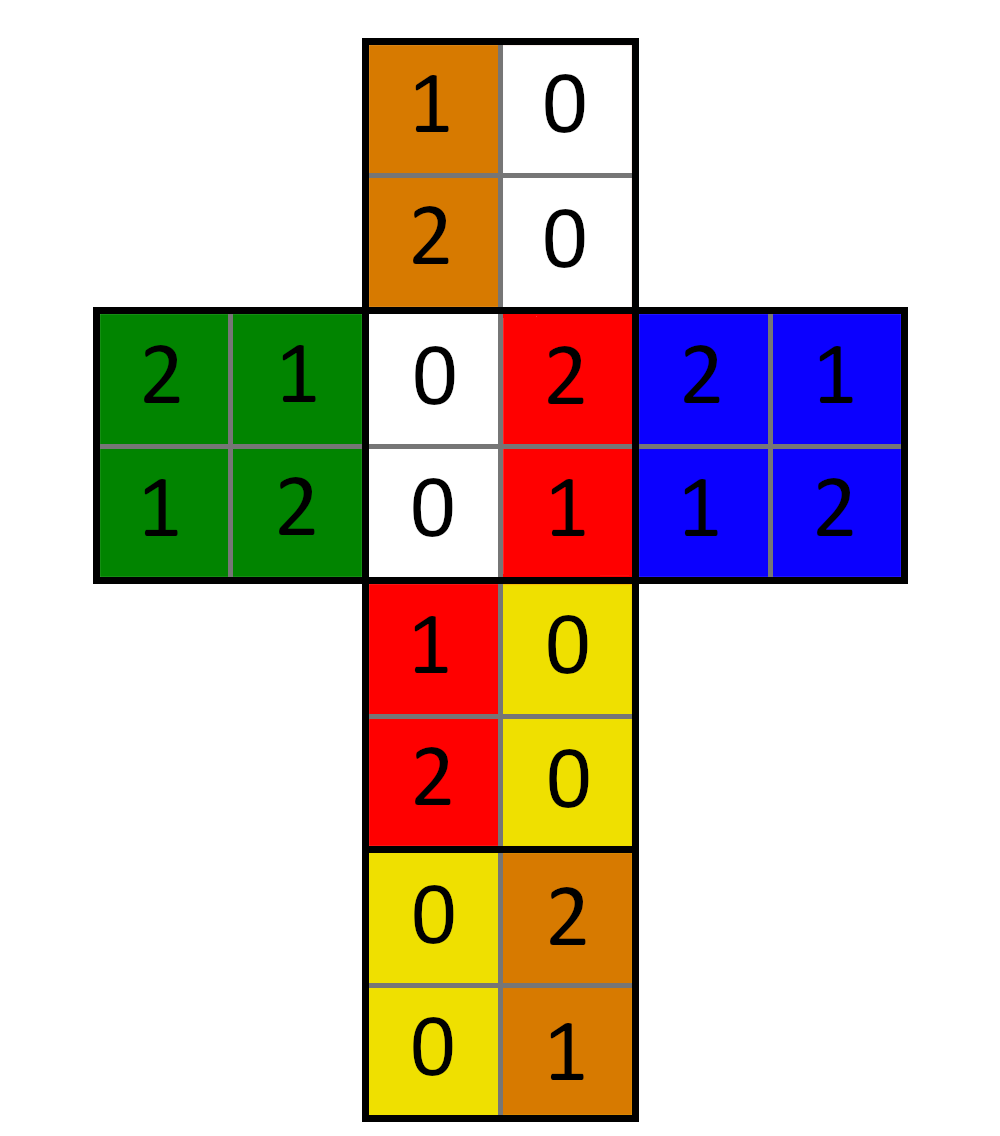
\includegraphics[scale=0.1]{foldedout_012_spin.png}
\caption{links: Positionen $x_1$ bis $x_8$, rechts: Veränderung der nummerierten Ecksteine nach dem Zug $R$}
\end{figure}
\ \\
\subsection*{Rotation des Würfels}


\section{Züge als Gruppenoperation}

Wenn der Zauberwürfel in einer Konfiguration $C=(\sigma, x)$ ist, wird der Würfel durch das Ausführen eines Zuges $M \in G_{2x2x2}$ in eine neue Konfiguration gebracht. Diese Konfiguration schreibe ich als $C \cdot M$. \\
\\
Definition einer Gruppenoperation mit der Gruppe $(G_{2x2x2}, \circ)$ und der Menge $C$:
\begin{itemize}
\item $\cdot: C \times G_{2x2x2} \rightarrow C$ mit $(c, g) \rightarrow c \cdot g $
\item $c \cdot N = x$ für alle $c \in C$ und das neutrale Element $N \in G_{2x2x2}$  
\item $c \cdot (u \circ v) = (c \cdot h) \cdot v$ für alle $u, v \in G_{2x2x2}$ und $c \in C$
\end{itemize}
\ \\
Angenommen der Würfel befindet sich in der Konfiguration $C$. Wenn nun der Zug $M_1 \in G_{2x2x2}$ ausgeführt wird, ist die neue Konfiguration des Würfels $C \cdot M_1$. Wenn nun noch ein weiterer Zug $M_2 \in G_{2x2x2}$ ausgeführt wird,ist die neue Konfiguration des Würfels $(C \cdot M_1) \cdot M_2$. \\
Anders gesagt: Der Würfel hat in Konfiguration $C$ gestartet und der Zug $M_1 M_2$ wurde ausgeführt. Man kann die neue Konfiguration alsl auch als $C \cdot (M_1 M_2)$ schreiben und somit gilt $(C \cdot M_1) \cdot M_2 = C \cdot (M_1 M_2)$. \\
\\
Wenn wir den leeren Zug $N$ ausführen, wird die Konfiguration des Würfels nicht verändert. Es gilt also $C \cdot N = C$. \\
\\
Bei Gruppenoperationen beeinflussen die Elemente einer Gruppe eine Menge. In diesem Fall beeinflussen die Züge des Würfels die Konfiguration des Würfels. \\
Es handelt sich hier um eine Rechtsoperation, da die Elemente der Gruppe rechts stehen. 

\section{Valide Konfigurationen des Würfels}
Die Konfiguration des Würfels ist definiert als $C=(\sigma, x)$. \\
\\
In diesem Abschnitt werde ich zeigen, dass bei einer validen Würfelkonfiguration $\Sigma \  x_i \equiv_3 0$ (modulo) gilt. \\
Wenn $C'=(\sigma', x')$ eine Nachfolgekonfiguration von $C=(\sigma, x)$ ist, dann gilt  $(\sigma, x) \cdot M = (\sigma', x')$. Dabei ist $M$ eine der Züge aus $U, D, R, L, F, B$. Es gilt dann $\Sigma x_i' \equiv_3 \Sigma \  x_i $. \\
In Abbildung 6 (s.o.) kann ist diese Situation für den Zug $R$ dargestellt. Das kann man auch anhand dieser Tabelle sehen: \\
\\
\begin{tabular}{|c|l|l|c|c|}
\hline
Zug $M$ & $x$ & $x'$ & $\Sigma \  x_i'$ & $\Sigma \  x_i' \equiv_3 0$ \\
\hline
\hline
\textit{D} & $(x_1, x_2, x_3, x_4, x_5, x_6, x_7, x_8)$ & $(x_1, x_2, x_3, x_4, x_6, x_8, x_5, x_7)$ & 0 & 0 \\
\hline
\textit{U} & $(x_1, x_2, x_3, x_4, x_5, x_6, x_7, x_8)$ & $(x_3, x_1, x_4, x_2, x_5, x_6, x_7, x_8)$ & 0 & 0 \\
\hline
\textit{R} & $(x_1, x_2, x_3, x_4, x_5, x_6, x_7, x_8)$ & $(x_1, 2, x_3, 1, x_5, 1, x_7, 2)$ & 6 & 0 \\
\hline
\textit{L} & $(x_1, x_2, x_3, x_4, x_5, x_6, x_7, x_8)$ & $(1, x_2, 2, x_4, 2, x_6, 1, x_8)$ & 6 & 0 \\
\hline
\textit{F} & $(x_1, x_2, x_3, x_4, x_5, x_6, x_7, x_8)$ & $(x_1, x_2, 1, 2, x_5, x_6, 2, 1)$ & 6 & 0 \\
\hline
\textit{B} & $(x_1, x_2, x_3, x_4, x_5, x_6, x_7, x_8)$ & $(2, 1, x_3, x_4, 1, 2, x_7, x_8)$ & 6 & 0 \\
\hline

\end{tabular}
\ \\ \\ \\ \\
Wenn es also eine valide Konfiguration $C'=(\sigma', x')$, für die gilt $\Sigma x_i' \equiv_3 0$, dann gibt es einen Zug $M \in G_{2x2x2}$, so dass $M \cdot C'$ die Steine in die richtigen Positionen bringt also $(1,x)$. \\
\\
Von dieser Konfiguration $(1,x)$ ausgehend gibt es einen Zug $M \in G_{2x2x2}$, so dass alle Eckstücke richtig ausgerichtet sind. Dann ergibt sich die Konfiguration $(1, 0)$ und alle Ecktsücke sind in der richtigen Ausrichtung und Position. Der Würfel befindet sich also in der Startkonfiguration. \\



\newpage

\subsection*{Zeitplan}

Die Bachelorarbeit ist auf 4 Monate ausgelegt, das sind circa 16 Wochen. \\
Der Zeitplan wird etwa wie folgt aussehen: \\
\\
\begin{itemize}
\item[Woche 1]
\item[Woche 2]
\item[Woche 3]
\item[Woche 4]
\item[Woche 5]
\item[Woche 6]
\item[Woche 7]
\item[Woche 8]
\item[Woche 9]
\item[Woche 10]
\item[Woche 11]
\item[Woche 12]
\item[Woche 13]
\item[Woche 14]
\item[Woche 15]
\item[Woche 16]
\end{itemize}


\newpage

\section{Quellen, Abbildungen, Tabellen etc.}
Ich habe das Paper \glqq Group Theory and the Rubik's Cube\grqq \  von Janet Chen als Quelle verwendet.\\ 
\\
Alle bisher verwendeteten Grafiken, Abbildungen und Tabellen habe ich selbst (mit GIMP, Photoshop oder LateX) erstellt, um Markennennungen zu vermeiden und eine einheitliche Darstellung zu gewährleisten.
% Alle verwendeten Abbildungen: \\
% \begin{figure}[H]
% 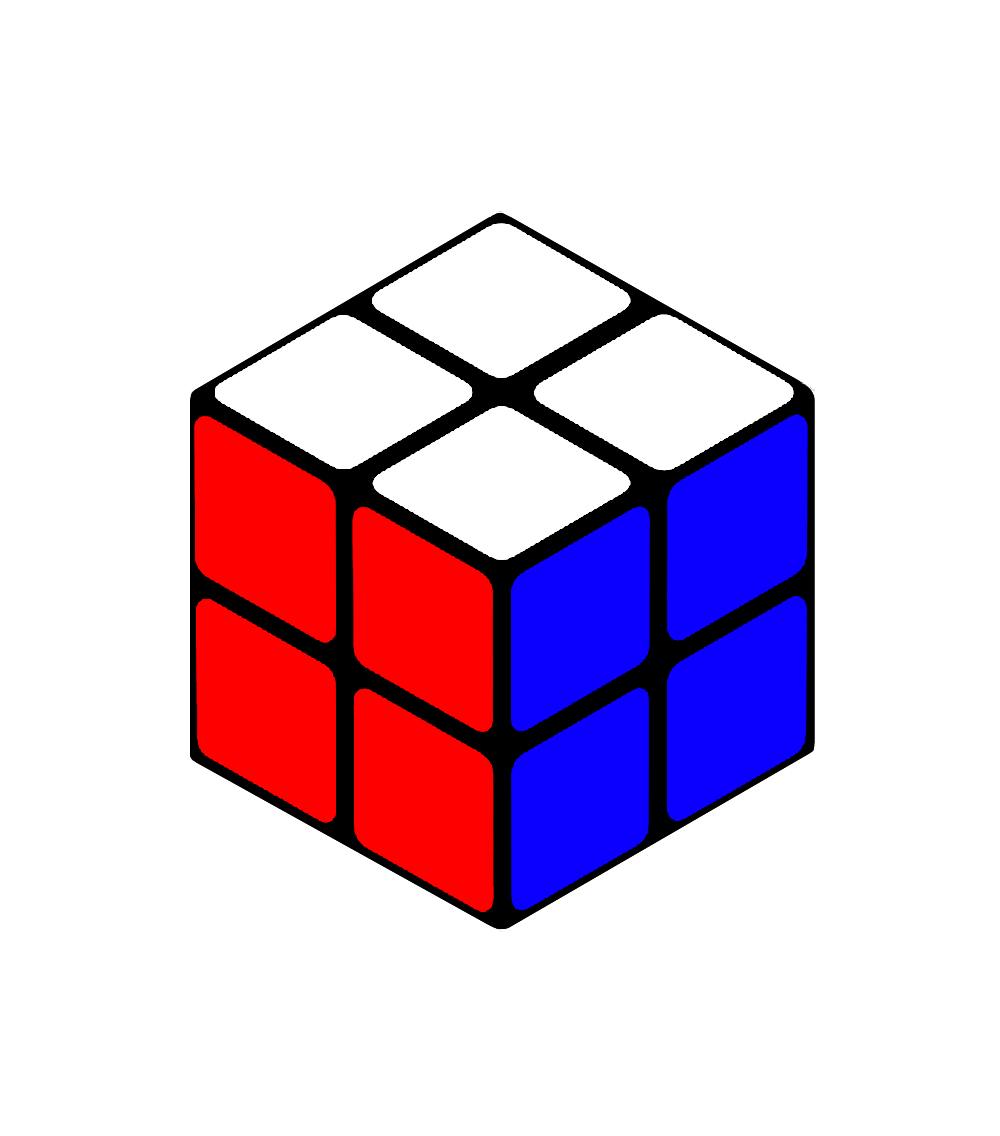
\includegraphics[scale=0.04]{2x2solved.png}
% 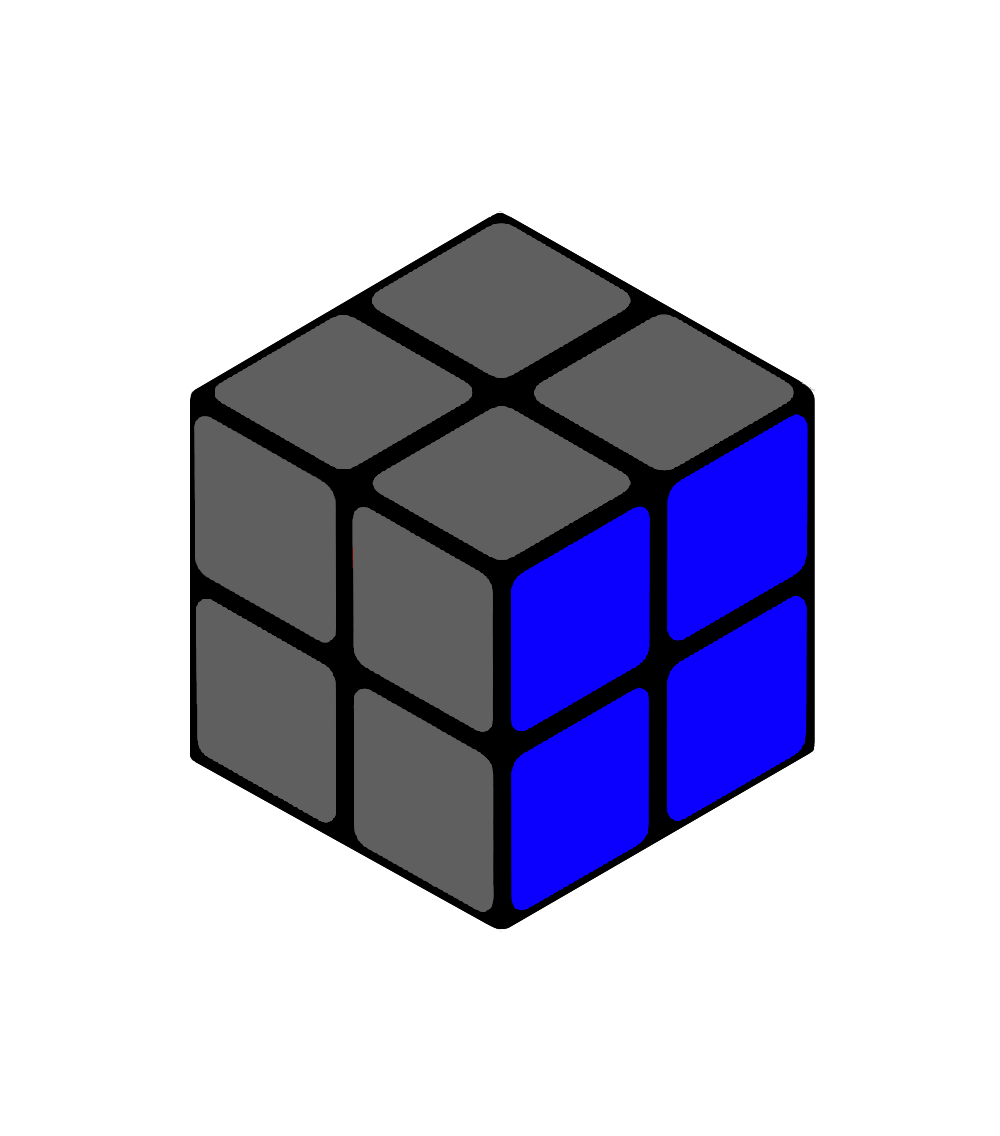
\includegraphics[scale=0.04]{2x2seite.png}
% 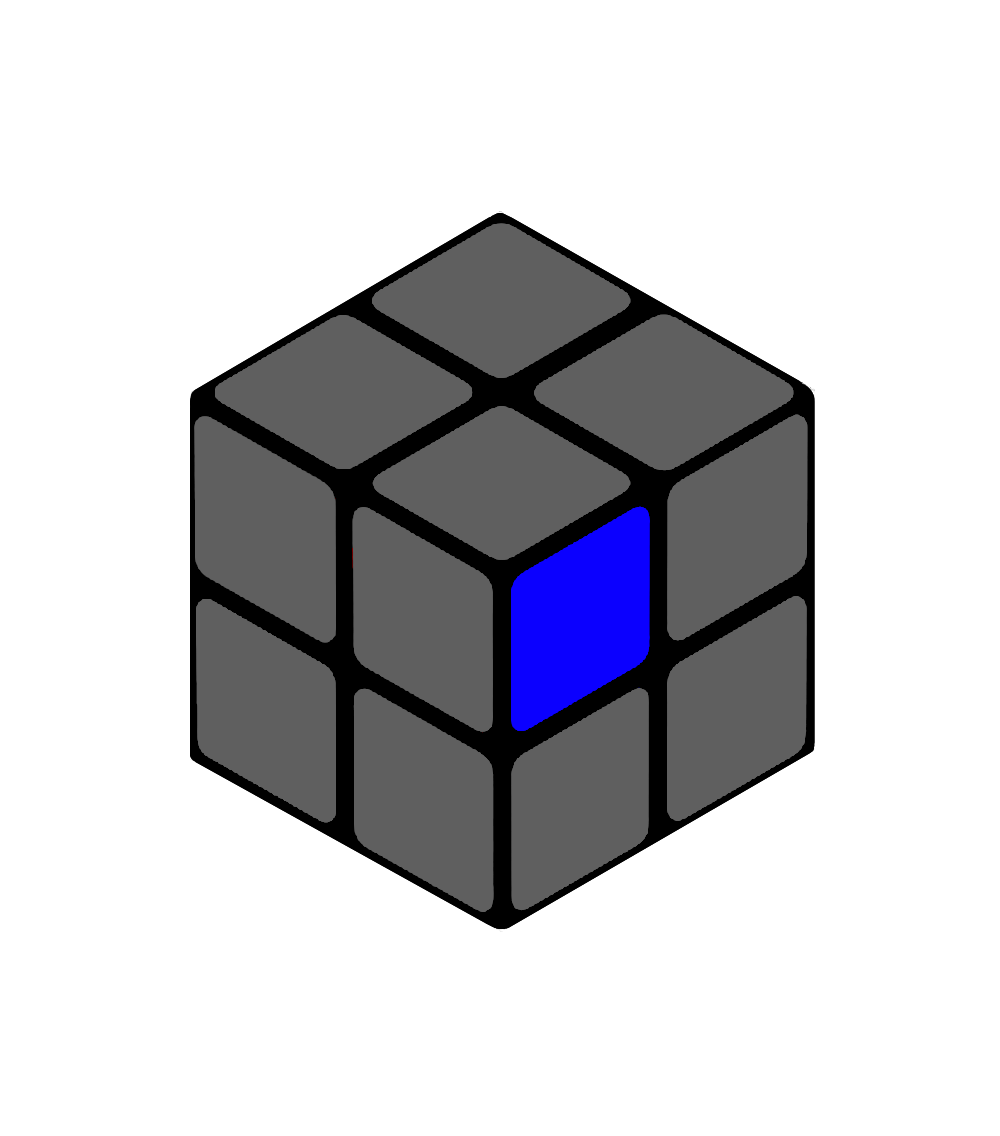
\includegraphics[scale=0.04]{2x2farbflaeche.png}
% 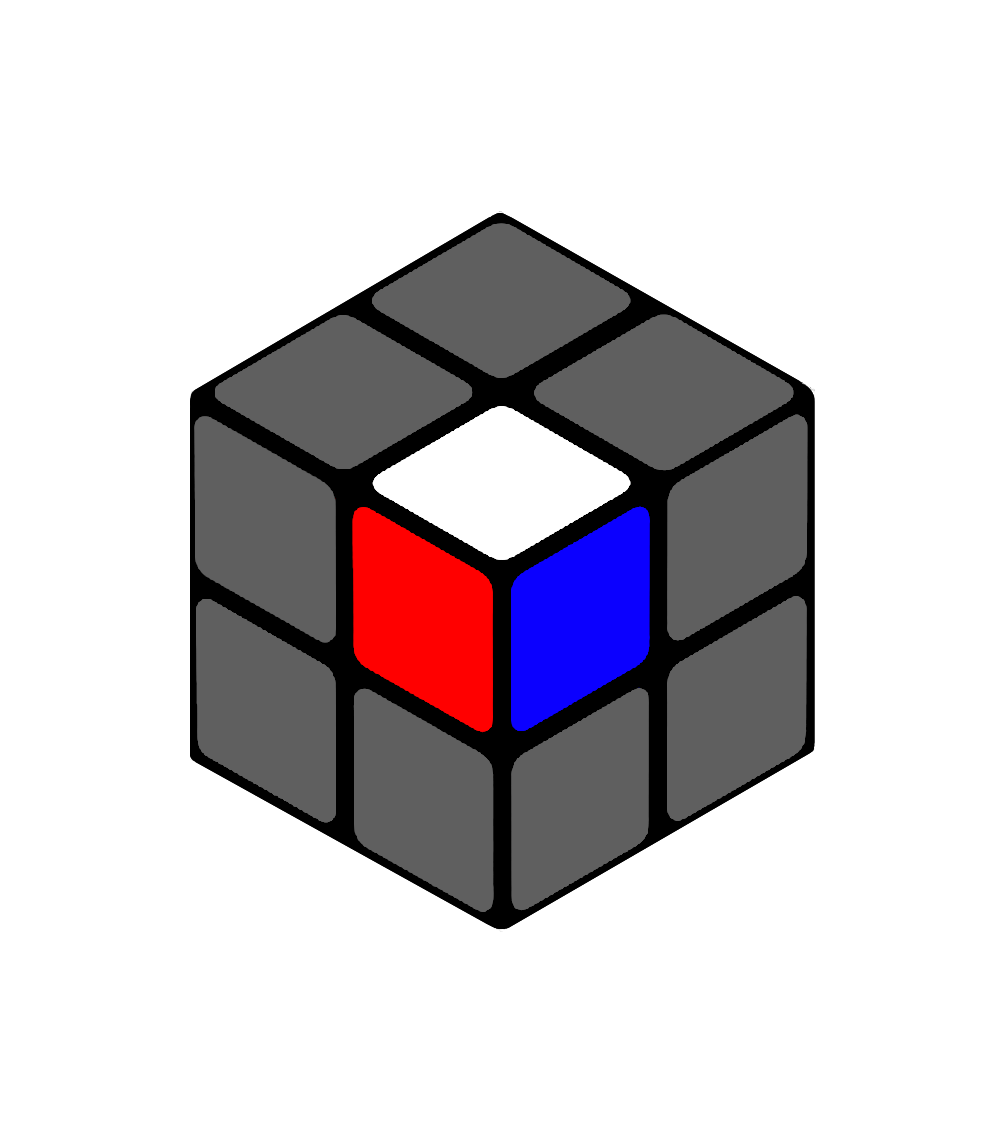
\includegraphics[scale=0.04]{2x2stein.png} 
% 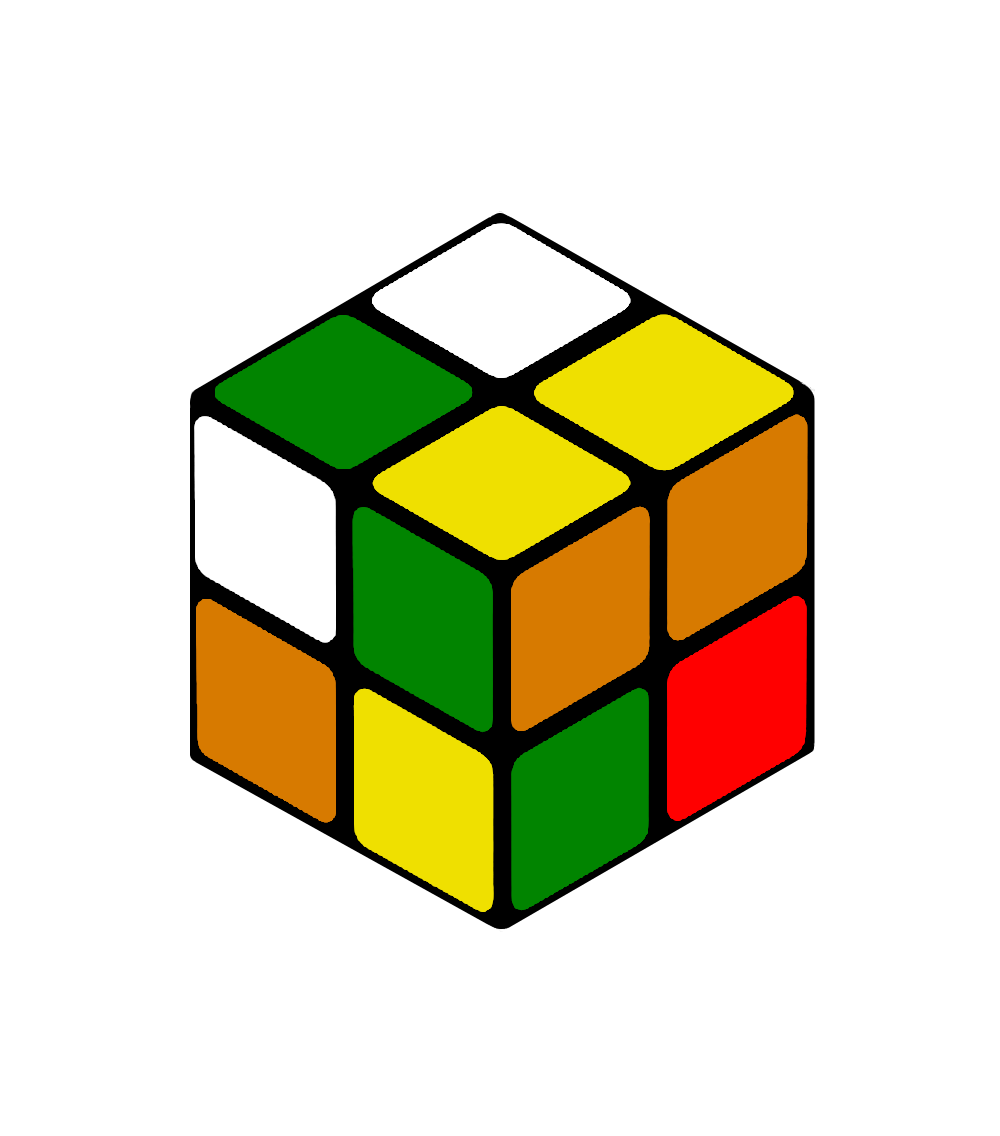
\includegraphics[scale=0.04]{2x2scrambled.png}
% 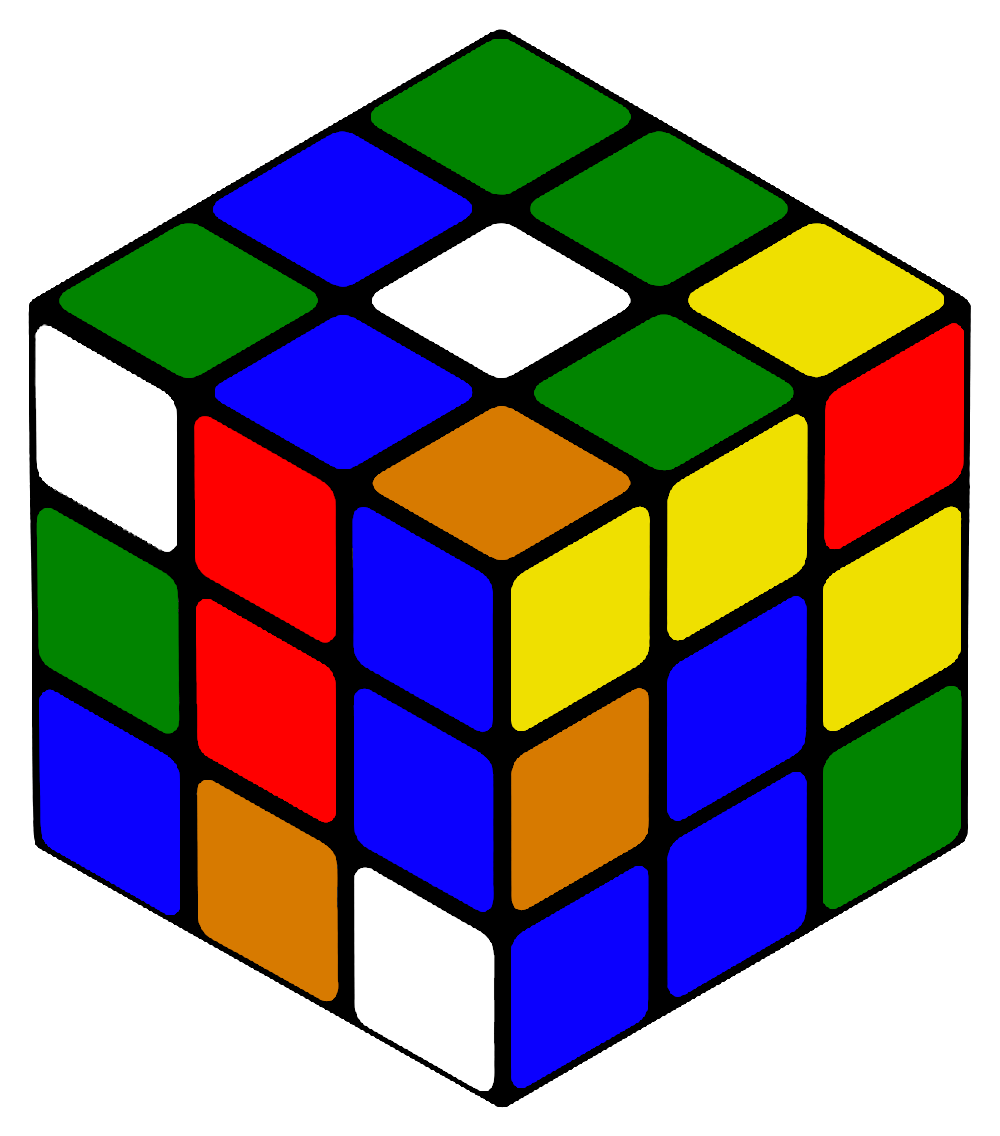
\includegraphics[scale=0.04]{3x3scrambled.png}
% 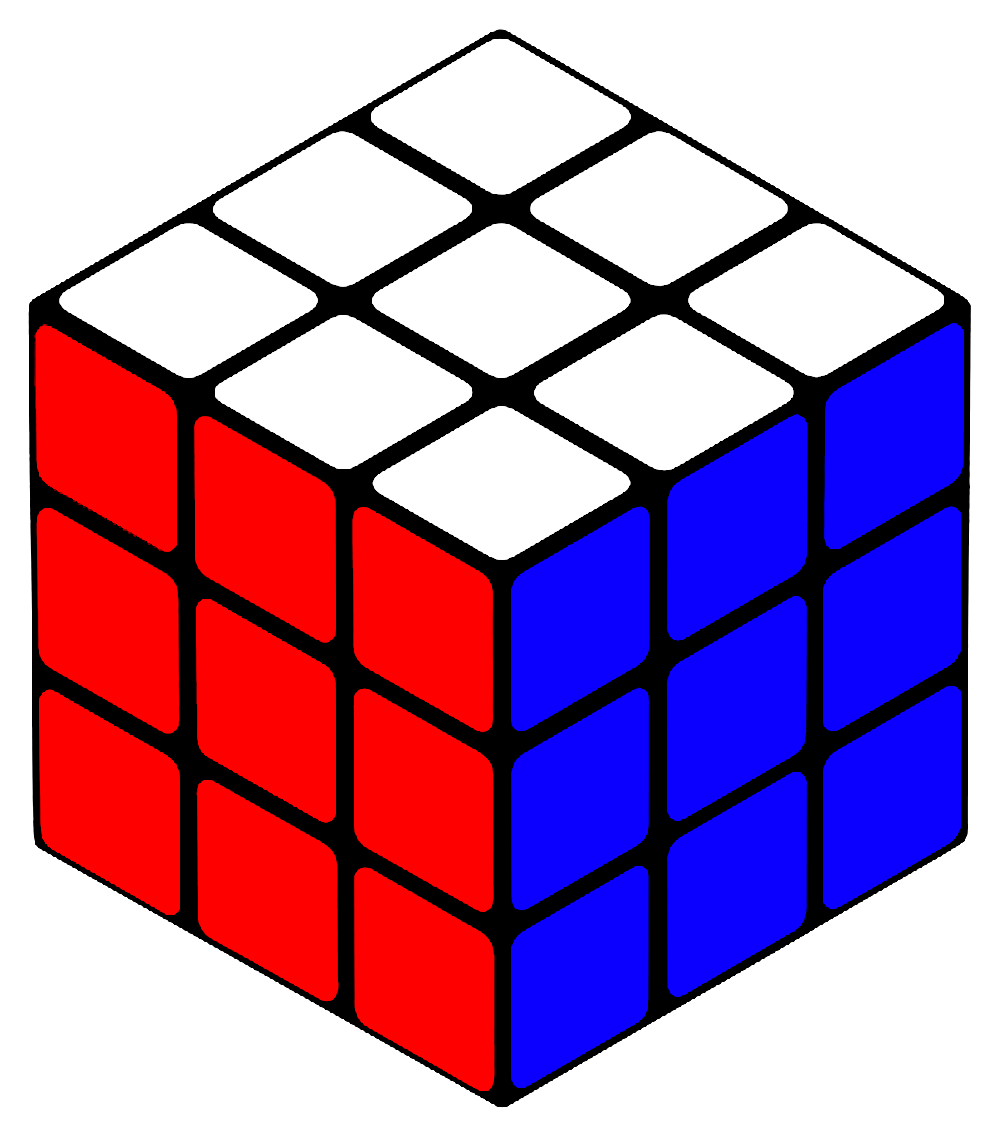
\includegraphics[scale=0.04]{3x3solved.png}
% 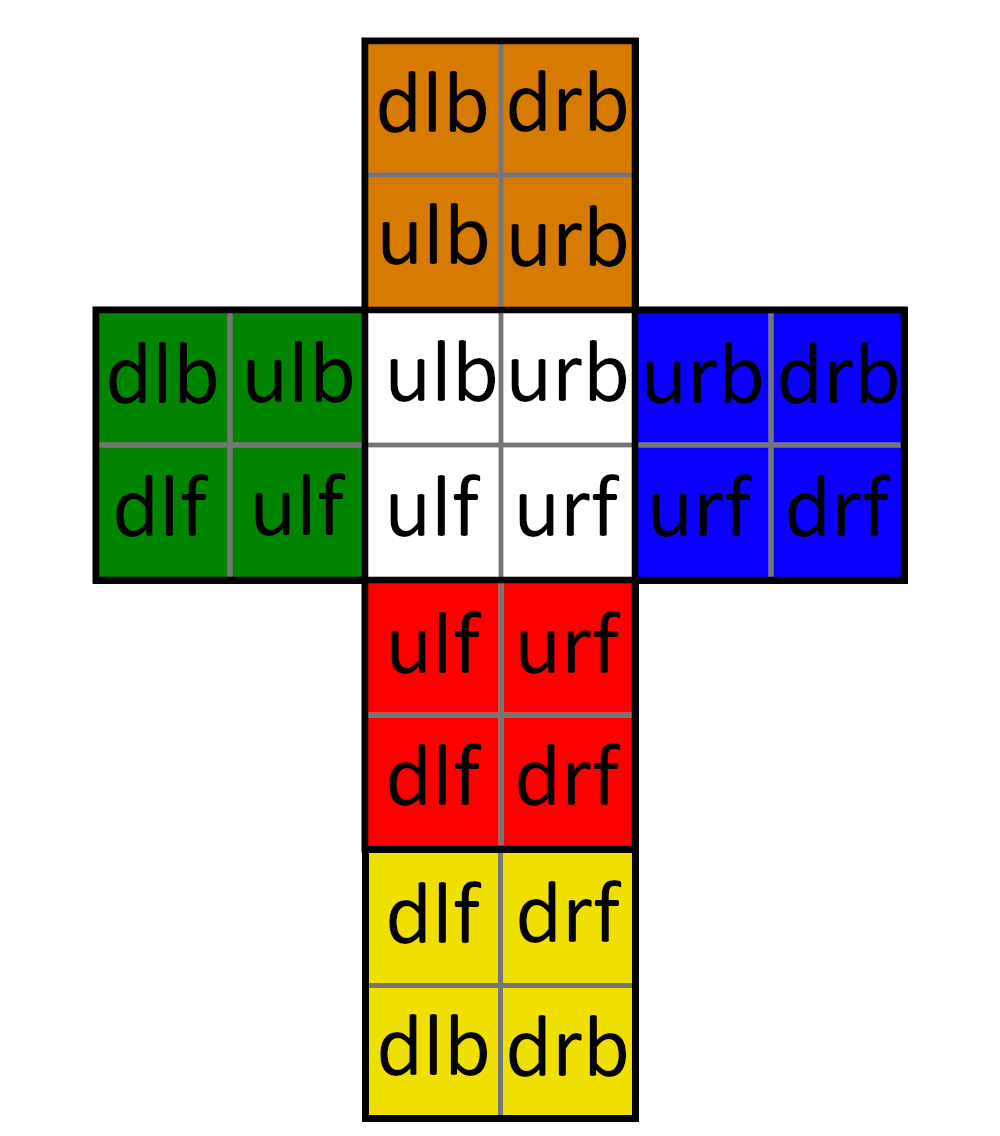
\includegraphics[scale=0.15]{foldedout_cage.png}
% 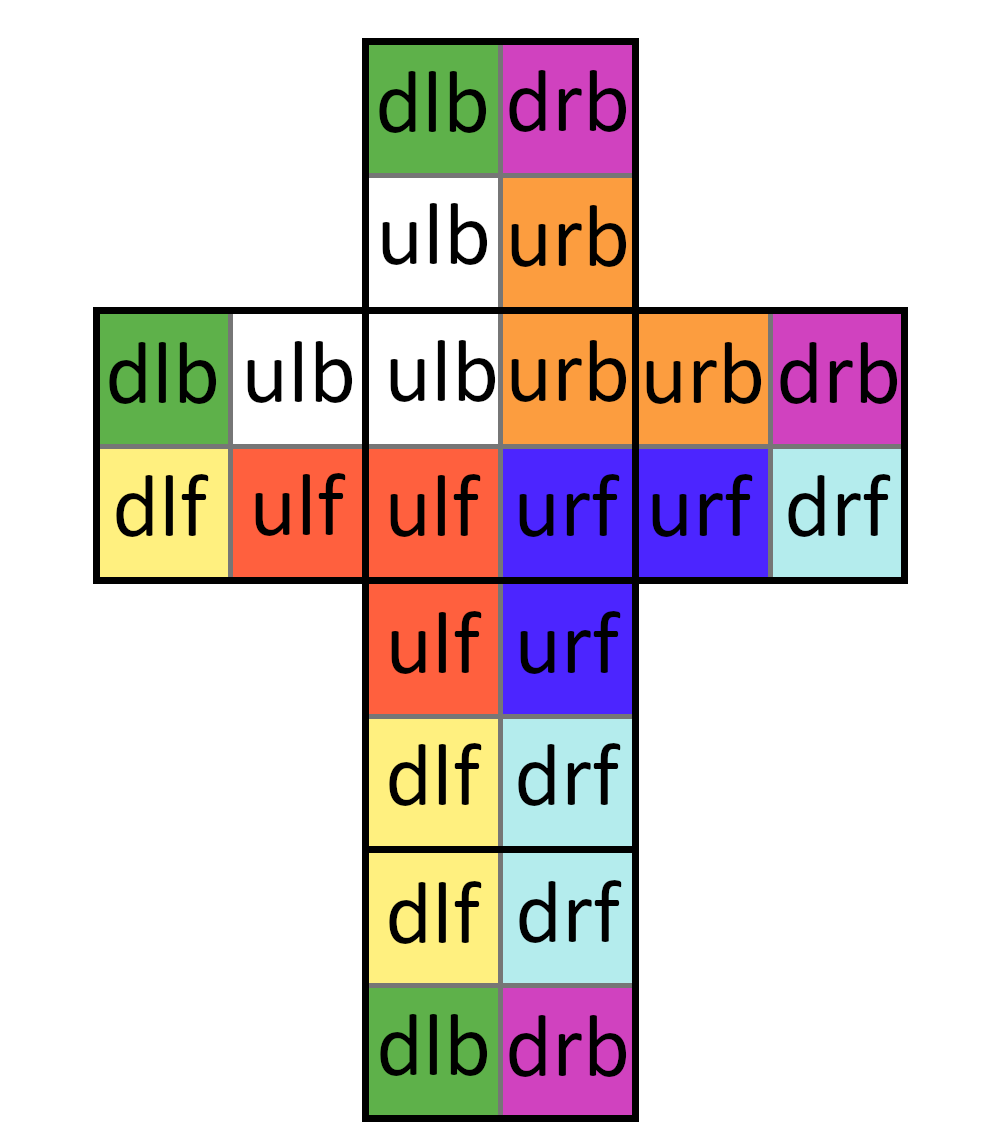
\includegraphics[scale=0.15]{foldedout_cage_color.png}
% 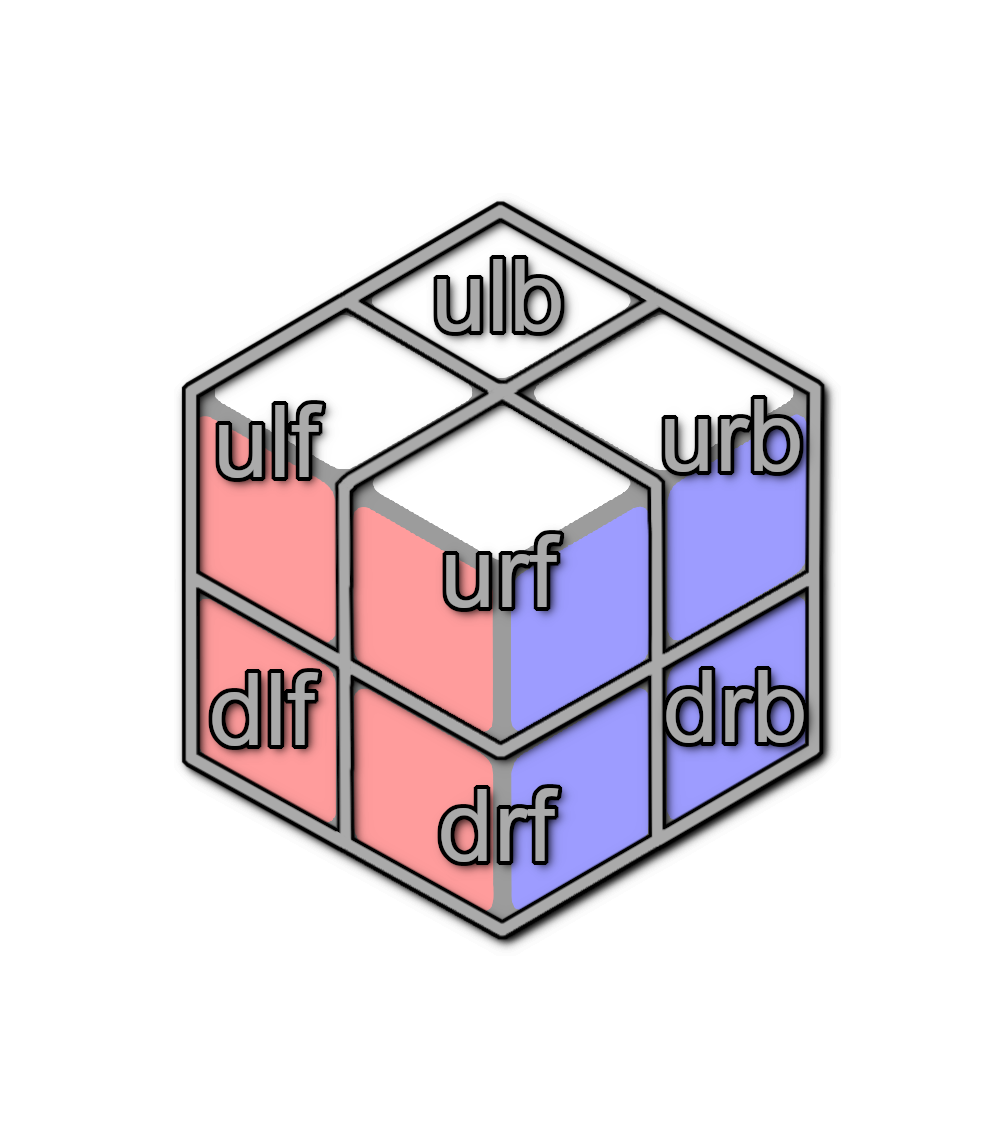
\includegraphics[scale=0.15]{caged_positions.png} 
% 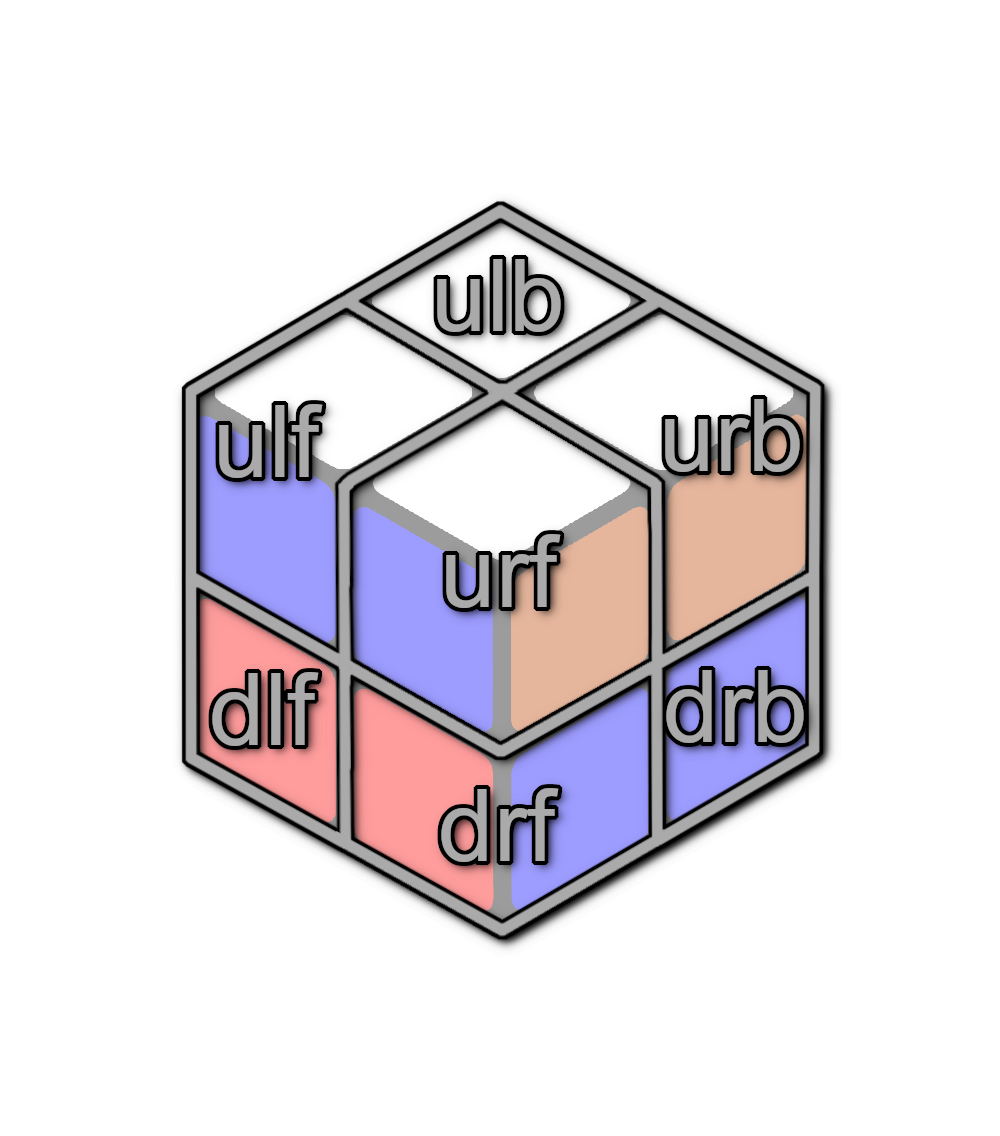
\includegraphics[scale=0.13]{caged_spin.png}
% 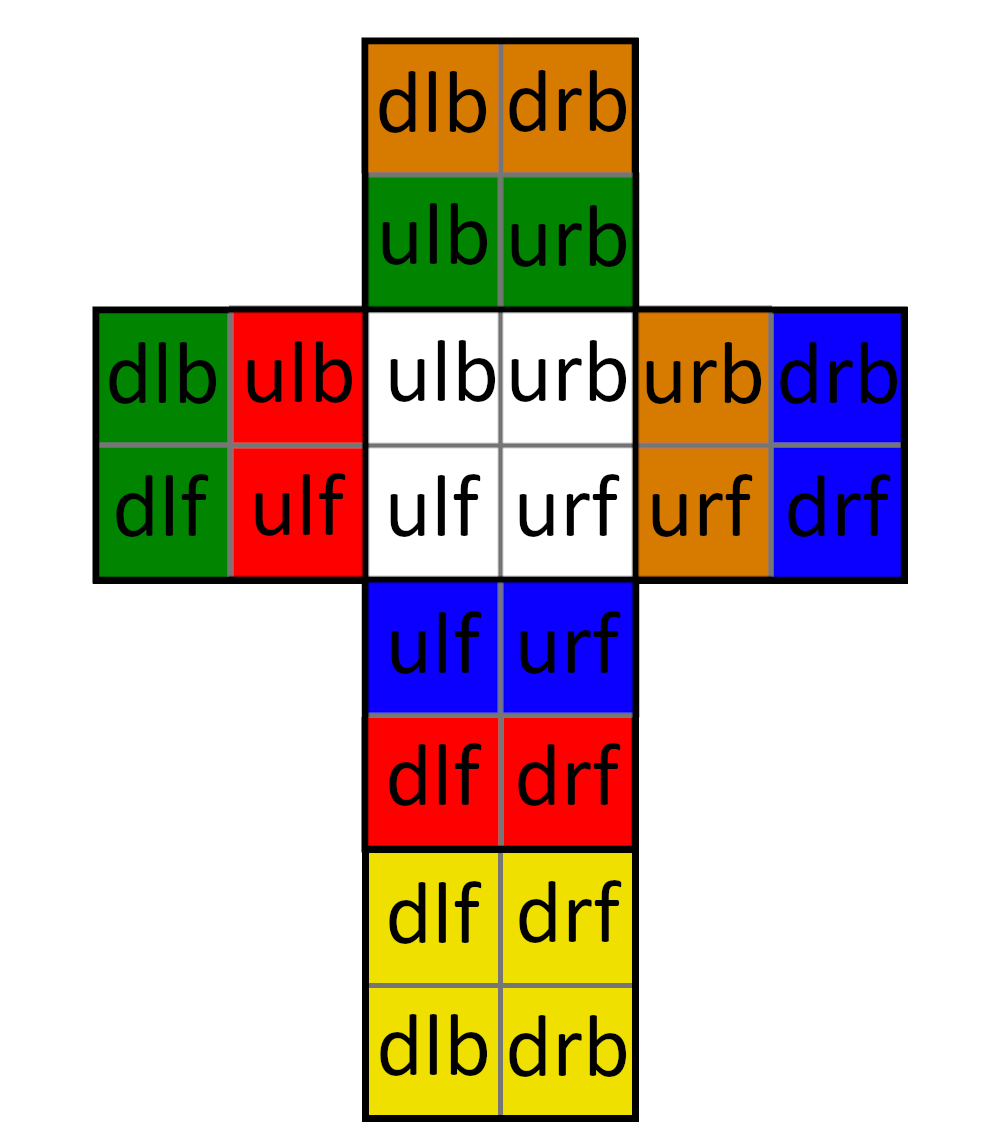
\includegraphics[scale=0.13]{foldedout_spin.png}
% 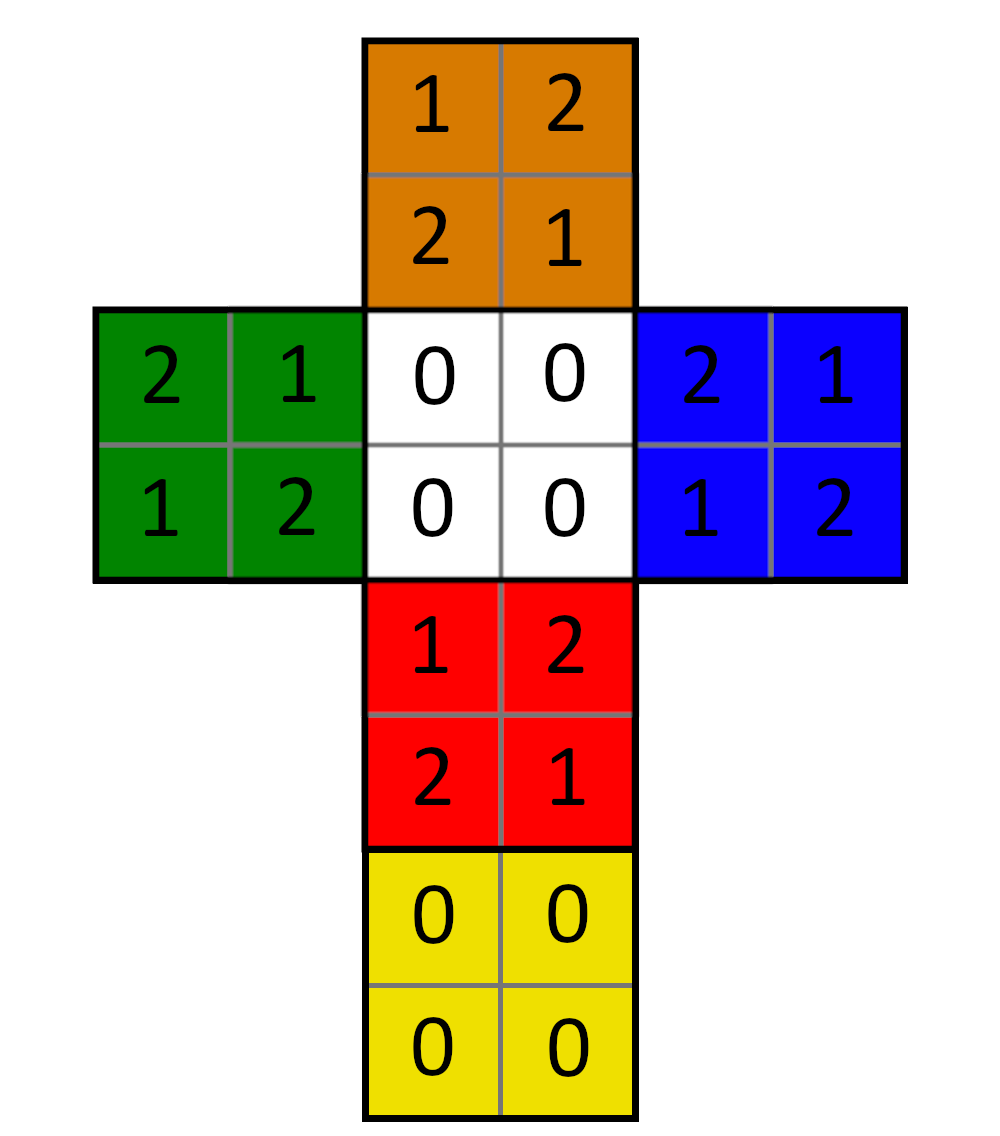
\includegraphics[scale=0.1]{foldedout_012.png}
% 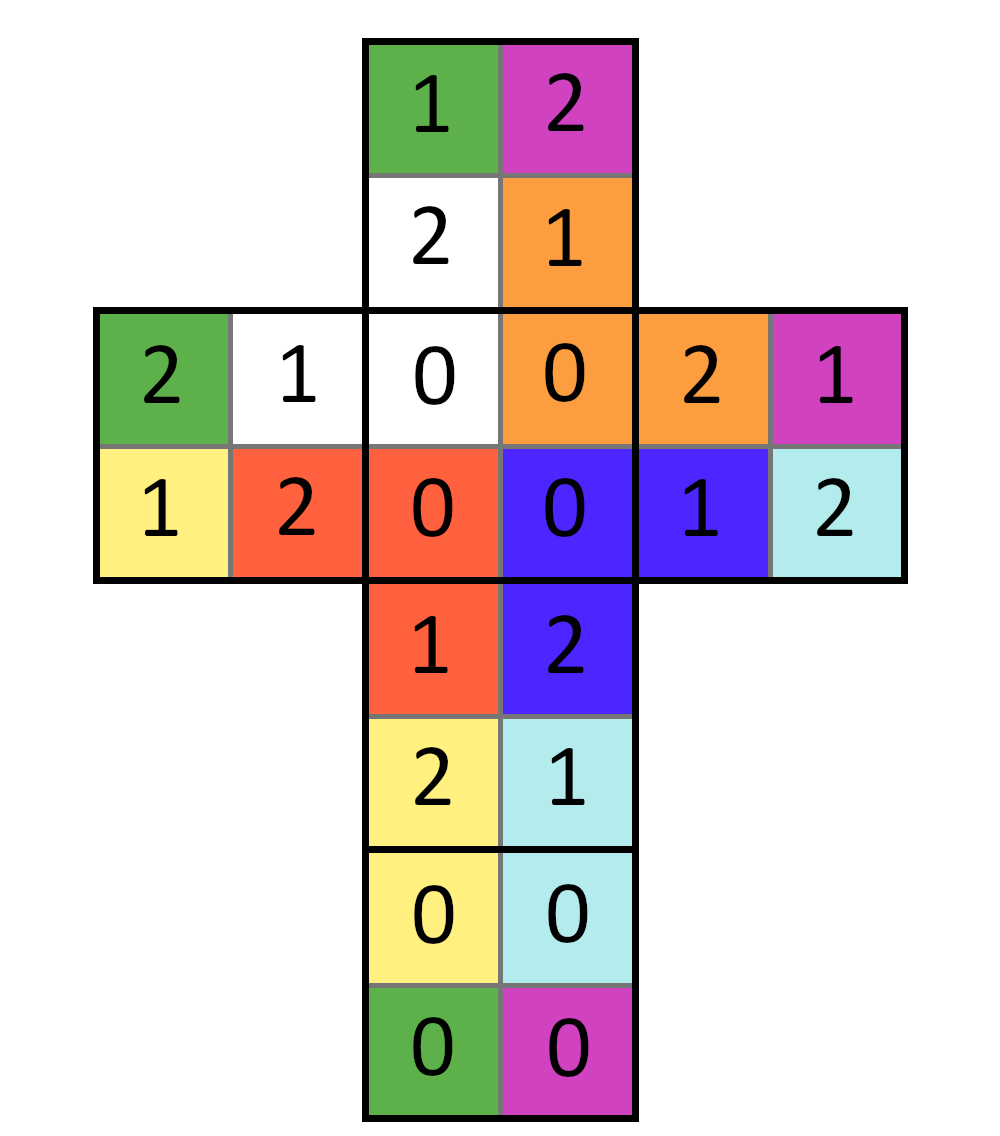
\includegraphics[scale=0.1]{foldedout_c_012.png}
%\end{figure}

\end{document}




